%%%%%%%%%%%%%%%%%%%%%%%%%%%%%%%%%%%%%%%%%%%%%%%%%%%%%%%%%%%%%%%%%%%%%%%%% 
% $Id$
% %%%%%%%%%%%%%%%%%%%%%%%%%%%%%%%%%%%%%%%%%%%%%%%%%%%%%%%%%%%%%%%%%%%%%%%%%
%
% Set de slides presentando el modulo fortran y sobre todo las lineas
% relevantes del fichero de entrada que tienen que ver con
% ello incluyendo el fichero de farfield.conf.
%
% Tambien se incluyen resultados del campo lejano con solucion
% analitica
% 
% %%%%%%%%%%%%%%%%%%%%%%%%%%%%%%%%%%%%%%%%%%%%%%%%%%%%%%%%%%%%%%%%%%%%%%%%%

  \begin{frame}[fragile,allowframebreaks]{Fortran Module}{\url{EMULATION_2D_scattering_module.F90}}

    \begin{lstlisting}[style=myFORTRANcodeS]
   TYPE :: EMULATION_2D_scattering_type
      PRIVATE 
      LOGICAL :: enabled_EMULATION_2D_scattering = &
           DEFAULT_ENABLED_EMULATION_2D_SCATTERING
      CHARACTER(len=2) :: green_function_type = DEFAULT_GREEN_FUNCTION_TYPE
      LOGICAL :: enabled_normal_incidence = DEFAULT_ENABLED_NORMAL_INCIDENCE
      ! Thickness (height) of 3D slice used to emulate 2D
      REAL(KIND=DBL) :: slice_thickness = DEFAULT_SLICE_THICKNESS 
   END TYPE EMULATION_2D_scattering_type

   PUBLIC ::  &
      is_EMULATION_2D_scattering_enabled, &
      enable_EMULATION_2D_scattering, &
      disable_EMULATION_2D_scattering, &
      get_EMULATION_2D_scattering_green_function_type, &
      set_EMULATION_2D_scattering_green_function_type, &
      is_EMULATION_2D_scattering_normal_incidence, &
      enable_EMULATION_2D_scattering_normal_incidence, &
      disable_EMULATION_2D_scattering_normal_incidence, &
      get_EMULATION_2D_scattering_slice_thickness, &
      set_EMULATION_2D_scattering_slice_thickness, &
      EMULATION_2D_scattering_print, &
      EMULATION_2D_scattering_sanitycheck         
    \end{lstlisting}


   \framebreak % %%%%%%%%%%%%%%%%%%%%%%%%%%

   
   \begin{block}{Input file \url{.em}} 
     \begin{lstlisting}[basicstyle=\ttfamily\footnotesize,tabsize=3,frame=none]
--------------------------------------
--     EMULATION 2D properties      --
--------------------------------------
-- EMULATION 2D activation flag
EMULATION_2D = true
-- Set the type of green function used
EMULATION_2D_green_function_type = "2D"
-- Activation flag for normal incidence
EMULATION_2D_normal_incidence = true
-- Thickness of the slice used as pseudo2D problem
EMULATION_2D_slice_thickness = 1.0
     \end{lstlisting}
   \end{block}

   \begin{itemize}
   \item The case of ``normal incidence'' is kept as a separate case
     \begin{itemize}
     \item It does not require periodic meshes
     \end{itemize}
   \item Value of ``slice thickness'' set up manually (desirable to be
     set automatically, e.g., GUI or HOFEM mesh preprocessing)
   \end{itemize}
   
  \end{frame}
  
% %%%%%%%%%%%%%%%%%%%%%%%%%%%%%%%%%%%%%%%%%%%%%%%%%%%%%%%%%%%%%%%
  
  \begin{frame}[fragile,allowframebreaks]{Fortran Module}{\url{EMULATION_2D_scattering_module.F90} }

    \begin{block}{Input file \url{.em}} 
      \begin{lstlisting}[basicstyle=\ttfamily\footnotesize,tabsize=3,frame=none]
--------------------------------------
--     EMULATION 2D properties      --
--------------------------------------
-- Orientation of the cylinder (axis unit vector)
EMULATION_2D_cylinder_axis = {0.0,1.0,0.0}
     \end{lstlisting}
   \end{block}


   \begin{itemize}
   \item Cylinder axis in arbitrary direction
     \begin{itemize}
     \item Cylinder axis is set up manually (desirable to be set
       automatically, e.g., GUI or HOFEM mesh preprocessing)
     \end{itemize}
   \end{itemize}     

   
   \framebreak % %%%%%%%%%%%%%%%%%%%%%%%%%%%%%%%%%%%%%
    \begin{block}{Input file \url{.em}} 
      \begin{lstlisting}[basicstyle=\ttfamily\footnotesize,tabsize=3,frame=none]
--------------------------------------
--     EMULATION 2D properties      --
--------------------------------------
-- Number of incidence angles to be analized
EMULATION_2D_num_exterior_excitations = 1
-- Type of plane wave ("Single", "Multiple")
EMULATION_2D_exterior_type_1 = "Single"
-- Angle of incidence (with respect to local spherical coordinate
-- system with z axis along the cylinder axis)
--   * First number is 'theta' (angle with respect to cylinder axis;
--     90 corresponds to normal incidence)
--   * Second number is 'phi' (angle of associated local cylindrical
--     coordinate system)
EMULATION_2D_exterior_angle_1 = {90,45}
-- Polarization (TM or TE)
EMULATION_2D_polarization_type_1 = "TM"
     \end{lstlisting}
   \end{block}

   \framebreak % %%%%%%%%%%%%%%%%%%%%%%%%%%%%%%%%%%%%%

   \begin{itemize}
   \item Definition of angles for excitations with respect to local
     spherical coordinate system with z axis along the cylinder axis
     \begin{itemize}
     \item Angles are transformed back and forth between local and
       global axis. 
     \end{itemize}

   \item Definition of polarization as either ``TM'' or ``TE''
     \begin{itemize}
     \item Vector components (polarization) are transformed back and
       forth between local and global axis.
     \end{itemize}

   \end{itemize}

   \framebreak % %%%%%%%%%%%%%%%%%%%%%%%%%%%%%%%%%%%%%


   \begin{block}{Input file \url{farfield_EMULATION_2D.conf}} 
      \begin{lstlisting}[basicstyle=\ttfamily\footnotesize,tabsize=3,frame=none]
!- Farfield mode (bistatic,monostatic)
Bistatic
!- Farfield component (|rE-longitudinal|, rE-longitudinal-real, rE-longitudinal-imag, rE-longitudinal-phase, |\
rE-transverse|, rE-transverse-real, rE-transverse-imag, rE-transverse-phase, RCS, RCS-transverse, RCS-longitud\
inal, RCS-dB, RCS-longitudinal-dB, RCS-transverse-dB, Monostatic-RCS, Monostatic-RCS-dB)
RCS
!- Frequency index and number of rhs
1 1
!- Rhs index
1
!- Rhs phase
0
!- Rhs amplitude
1
     \end{lstlisting}
   \end{block}

   \framebreak % %%%%%%%%%%%%%%%%%%%%%%%%%%%%%%%%%%%%%


   \begin{block}{Input file \url{farfield_EMULATION_2D.conf}} 
      \begin{lstlisting}[basicstyle=\ttfamily\footnotesize,tabsize=3,frame=none]
!- Monitor number
1
!- Phi_cyl sampling points (num init stop)
37 0 360
!- RCS units                             
sigma-lambda
!- Array analysis (flag,num_elem_u,num_elem_v) 
0 1 1                                                                            
     \end{lstlisting}
   \end{block}

   \framebreak % %%%%%%%%%%%%%%%%%%%%%%%%%%%%%%%%%%%%%
   
   \begin{itemize}
   \item Specialization to EMULATION 2D mode
     \begin{itemize}
     \item Farfield-mode: only scattering %(no ``Antenna'' support??)
     \item Farfield-component: ``longitudinal'' and ``transverse''
       components with respect to cylinder
     \item \ldots
     \end{itemize}
     
   \item Only the angles ``phi'' need to be defined for the plot (plot
     asociated to the transversal plane to the cylinder (perpendicular
     to its axis)

   \item Array analysis: we keep it as it might be of interest to
     consider finite 1D/2D periodic structures based on pseudo2D
     cylinders

   \end{itemize}


  \end{frame}

  
% %%%%%%%%%%%%%%%%%%%%%%%%%%%%%%%%%%%%%%%%%%%%%%%%%%%%%%%%%%%%%%%


  \begin{frame}[fragile,allowframebreaks]{Fortran Module}{\url{EMULATION_2D_scattering_module.F90} }

    \begin{itemize}
    \item Near field: {GreenD} derivatives are rewritten in a compact way
      supporting computation of the scattering near field (within
      FE-IIEE loop) for arbitraily oriented cylinders

    \item Far field: Perfect agreement between numerical and analytical
      solutions
      \begin{itemize}
      \item Well\ldots agreement up to a constant (not worried at all about it)
      \end{itemize}
    \end{itemize}

  \end{frame}


  
% %%%%%%%%%%%%%%%%%%%%%%%%%%%%%%%%%%%%%%%%%%%%%%%%%%%%%%%%%%%%%%%

% RESULTS  
% Far-field comparison (PEC and Coated PEC) with analytical solution

  \begin{frame}{Far-field Bistatic RCS calculation}{Reference cases}

The same geometry is analized with different orientations of the longitudinal axis:

\vbs

\begin{columns}

\column{0.4\textwidth}
\includegraphics[width=\linewidth]
{results/3D/20/300/\meshCCC{01}{1}{075}/geometry.pdf}

\column{0.55\textwidth}

\begin{itemize}

\item Normal incidence
\item Dashed black line:
\item Blue line: $S'$
\item Red line: $S$
\item Different values of permittivity between PEC and $S'$: $\varepsilon_r$
\item $f=300$\,MHz ($\lambda=1$\,m, cylinder radius is $5\lambda$).

\end{itemize}

\end{columns}

\end{frame}

\begin{frame}{TM polarization, $\varepsilon_r=1$ (reference case)}


\begin{columns}
\column{0.23\textwidth}

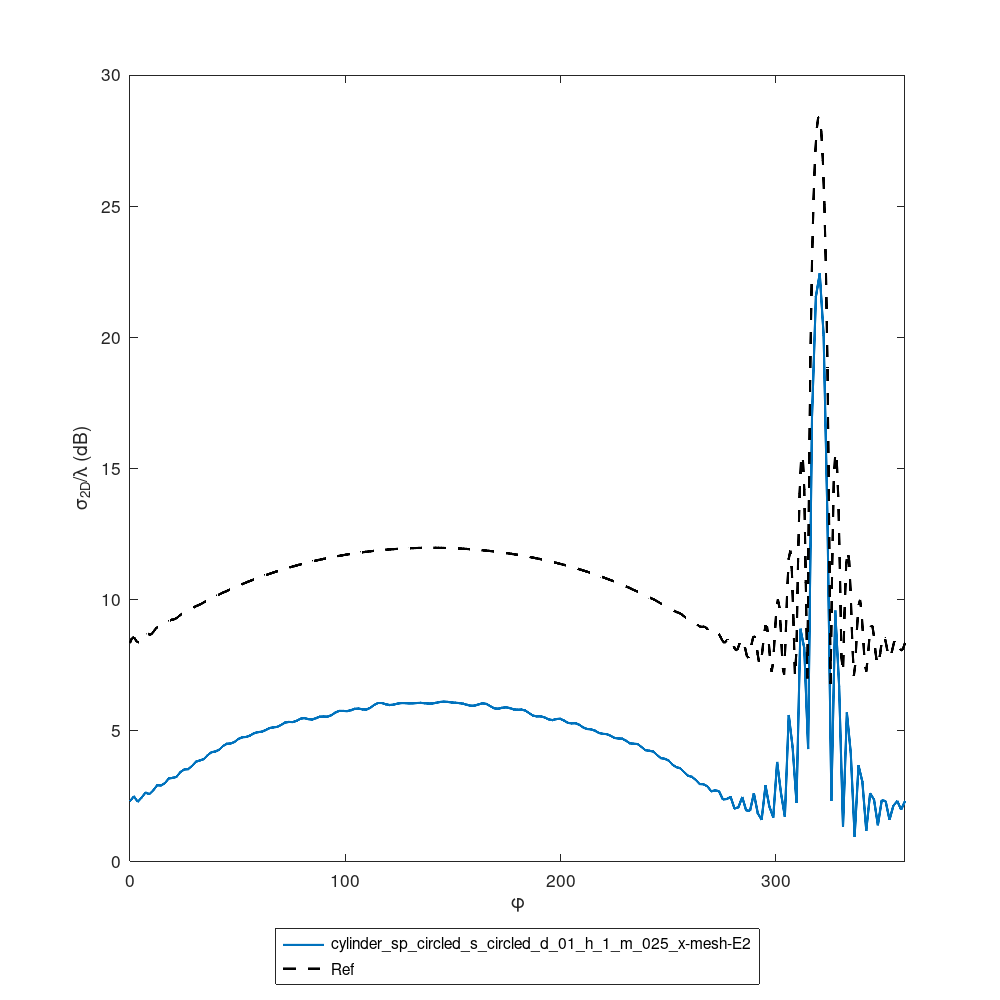
\includegraphics[width=\linewidth]{results/FF/cylD_01_H_1_M_025_X/iiee.png}

\column{0.23\textwidth}

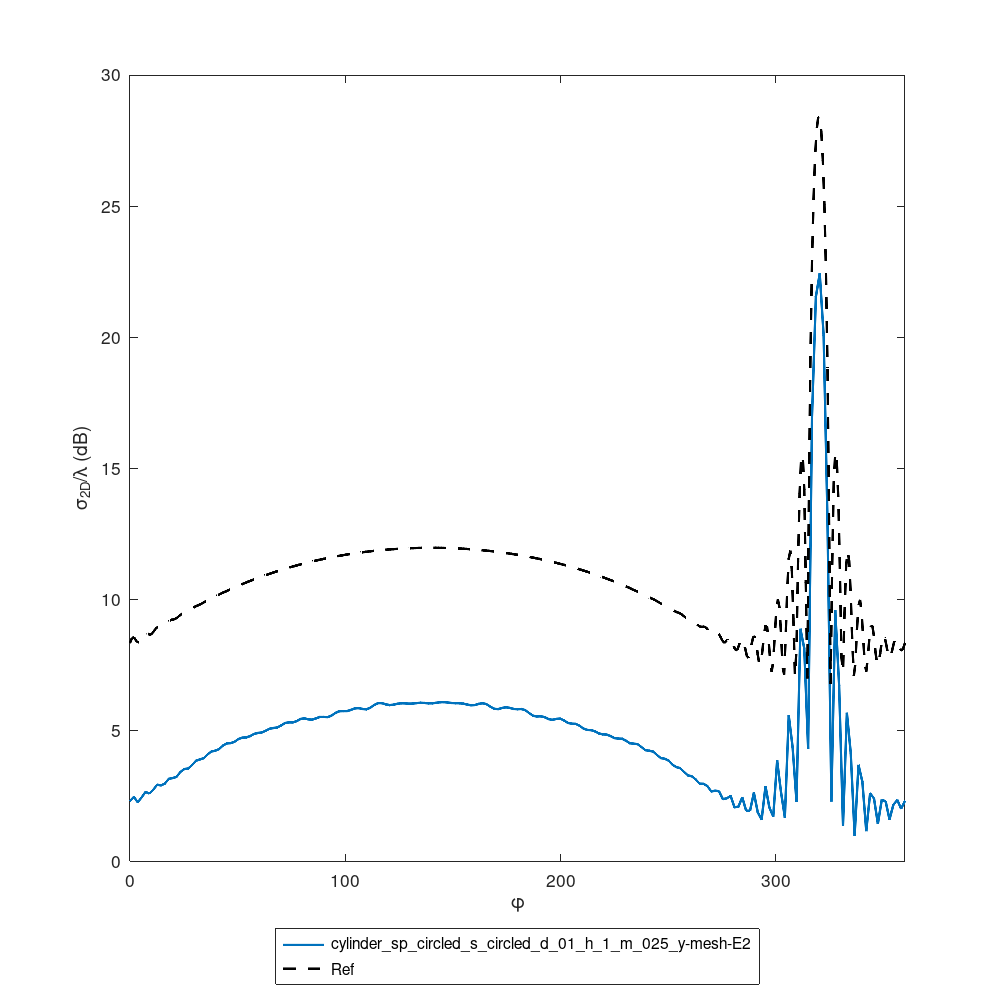
\includegraphics[width=\linewidth]{results/FF/cylD_01_H_1_M_025_Y/iiee.png}

\column{0.23\textwidth}

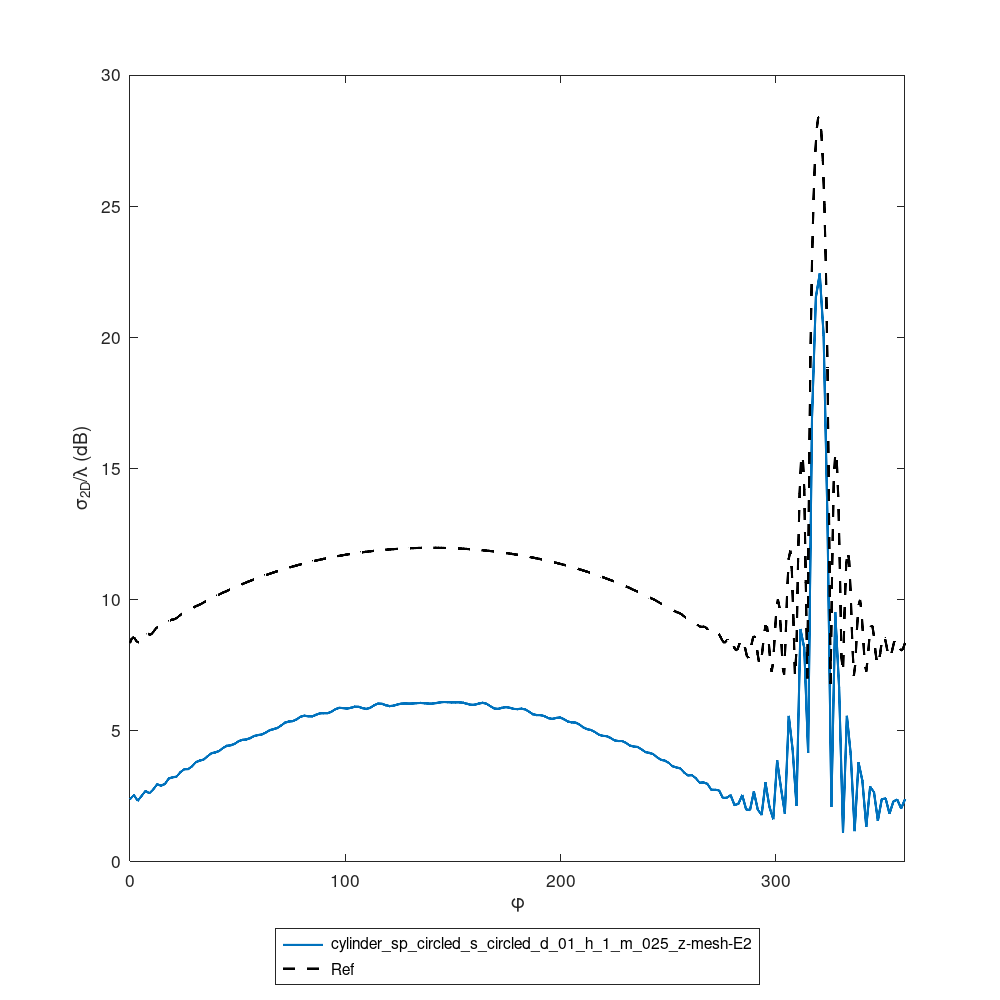
\includegraphics[width=\linewidth]{results/FF/cylD_01_H_1_M_025_Z/iiee.png}

\column{0.23\textwidth}

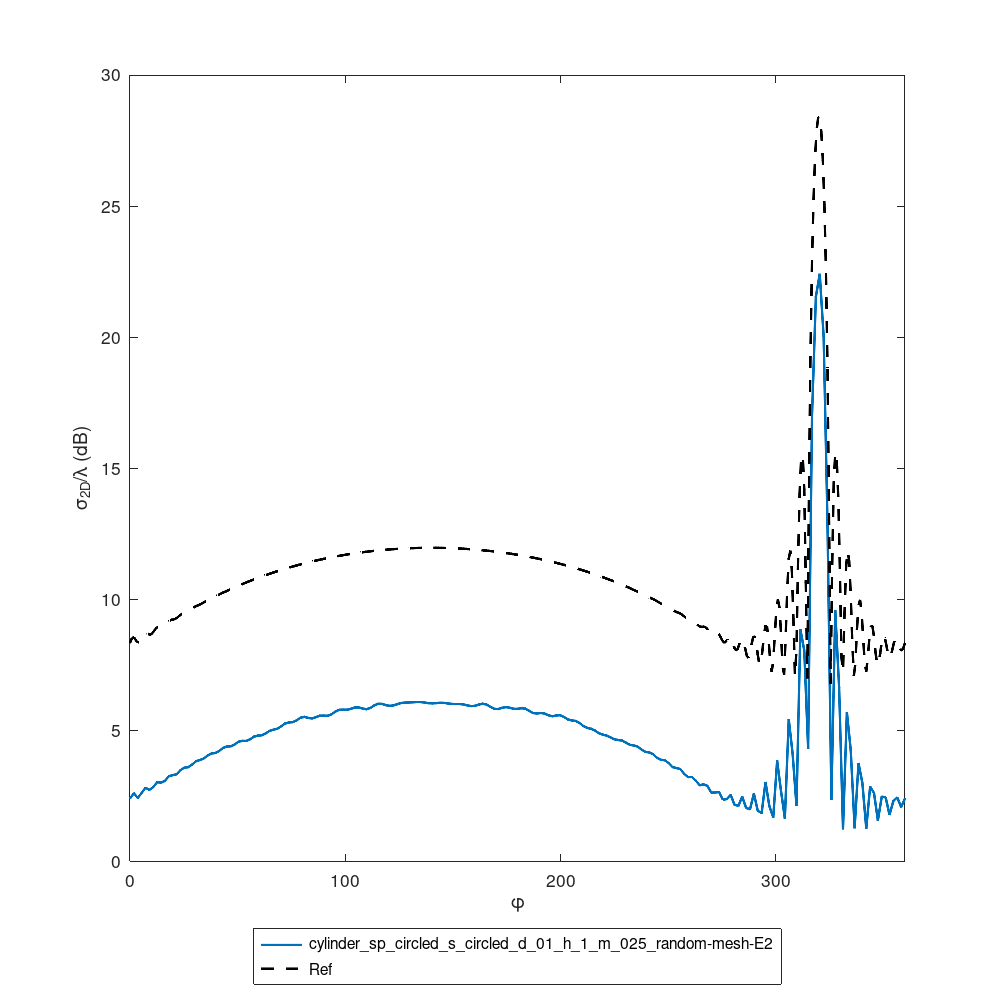
\includegraphics[width=\linewidth]{results/FF/cylD_01_H_1_M_025_RANDOM/iiee.png}

\end{columns}

\vbs

Analytical curves and FEM curves agree except for a constant factor. 

Normalized bistatic-RCS:

\vbss

\begin{columns}
\column{0.23\textwidth}

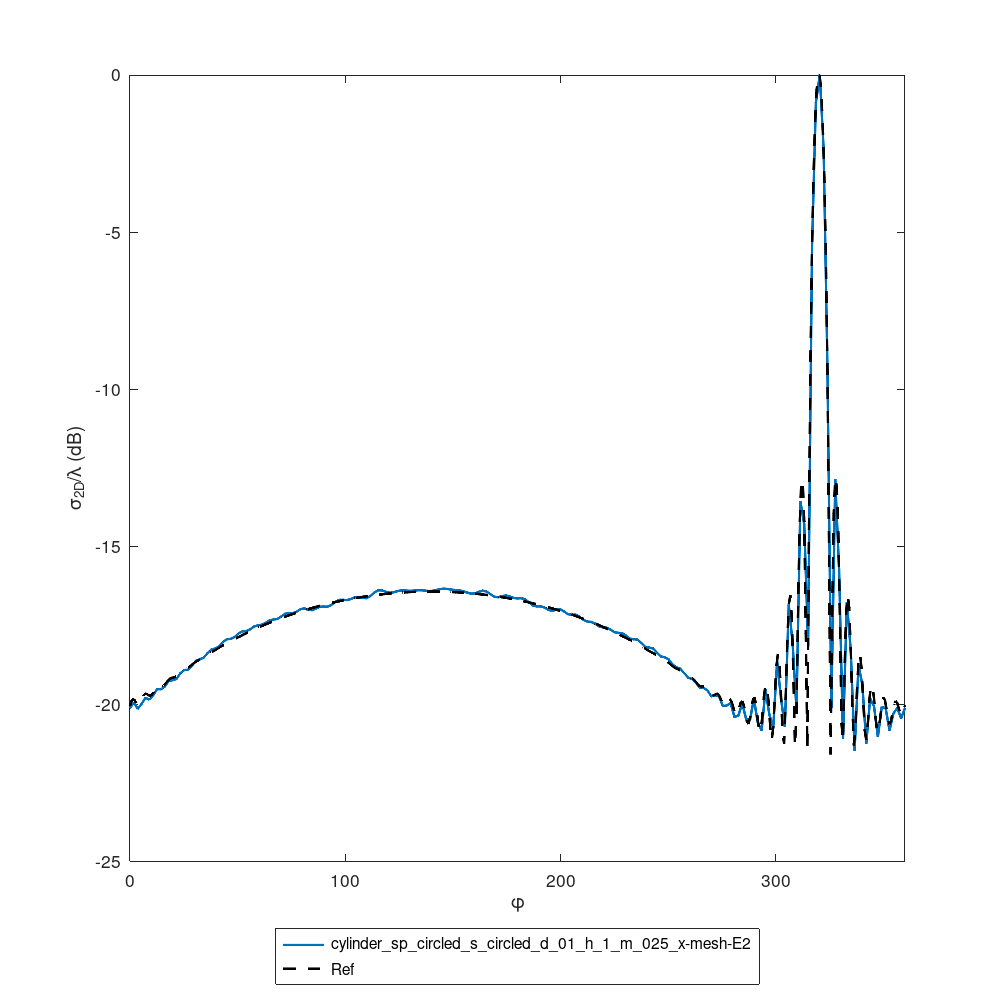
\includegraphics[width=\linewidth]{results/FF/cylD_01_H_1_M_025_X/iiee_norm.png}

\column{0.23\textwidth}

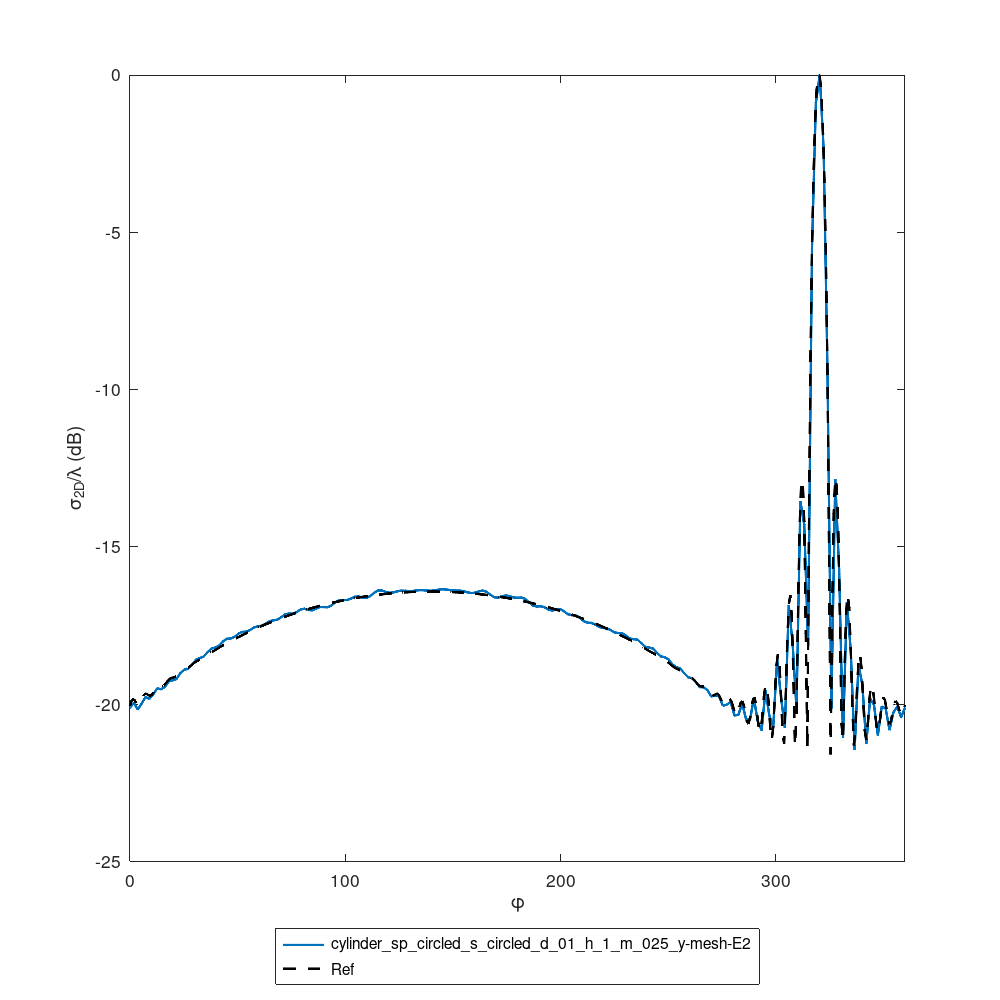
\includegraphics[width=\linewidth]{results/FF/cylD_01_H_1_M_025_Y/iiee_norm.png}

\column{0.23\textwidth}

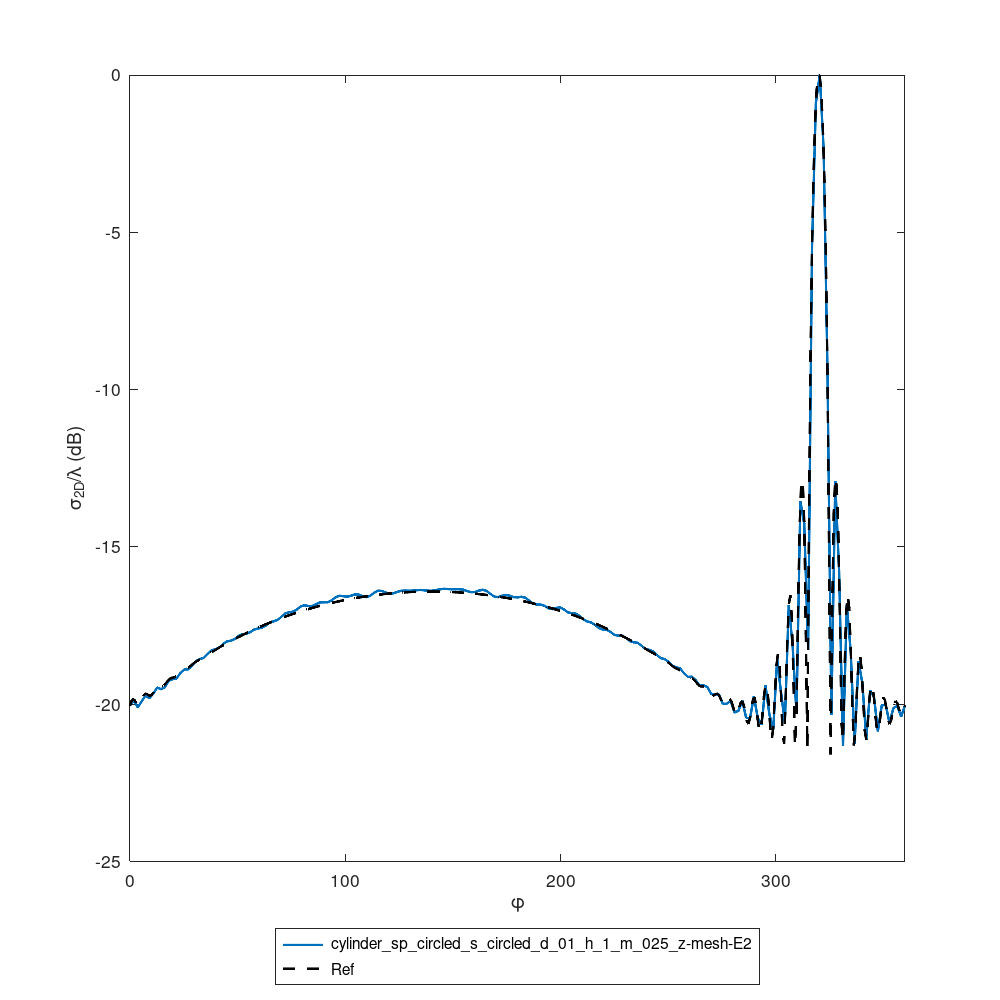
\includegraphics[width=\linewidth]{results/FF/cylD_01_H_1_M_025_Z/iiee_norm.png}

\column{0.23\textwidth}

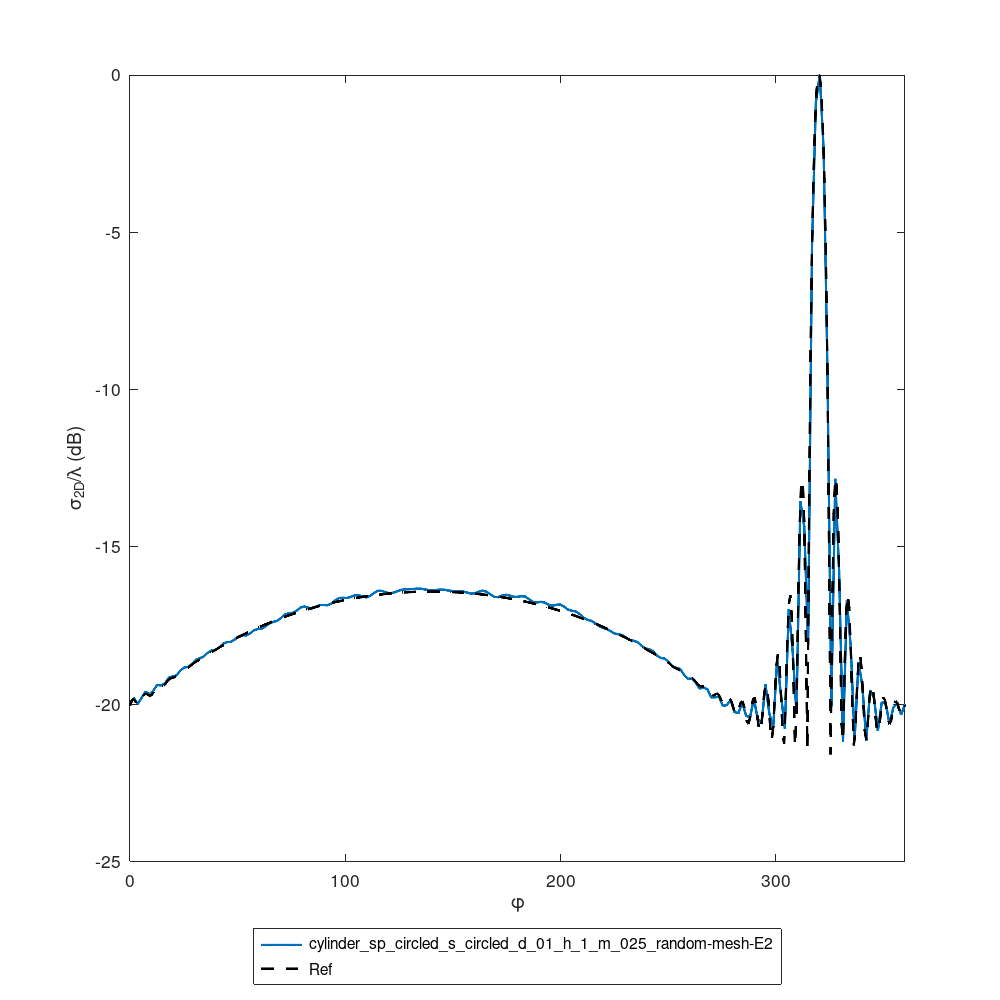
\includegraphics[width=\linewidth]{results/FF/cylD_01_H_1_M_025_RANDOM/iiee_norm.png}

\end{columns}


\end{frame}

%%%%%%%%%%%%%%%%%%%%%%%%%%%%%%%%%%%%%%%%

\begin{frame}{TE polarization, $\varepsilon_r=1$}

\begin{columns}
\column{0.23\textwidth}

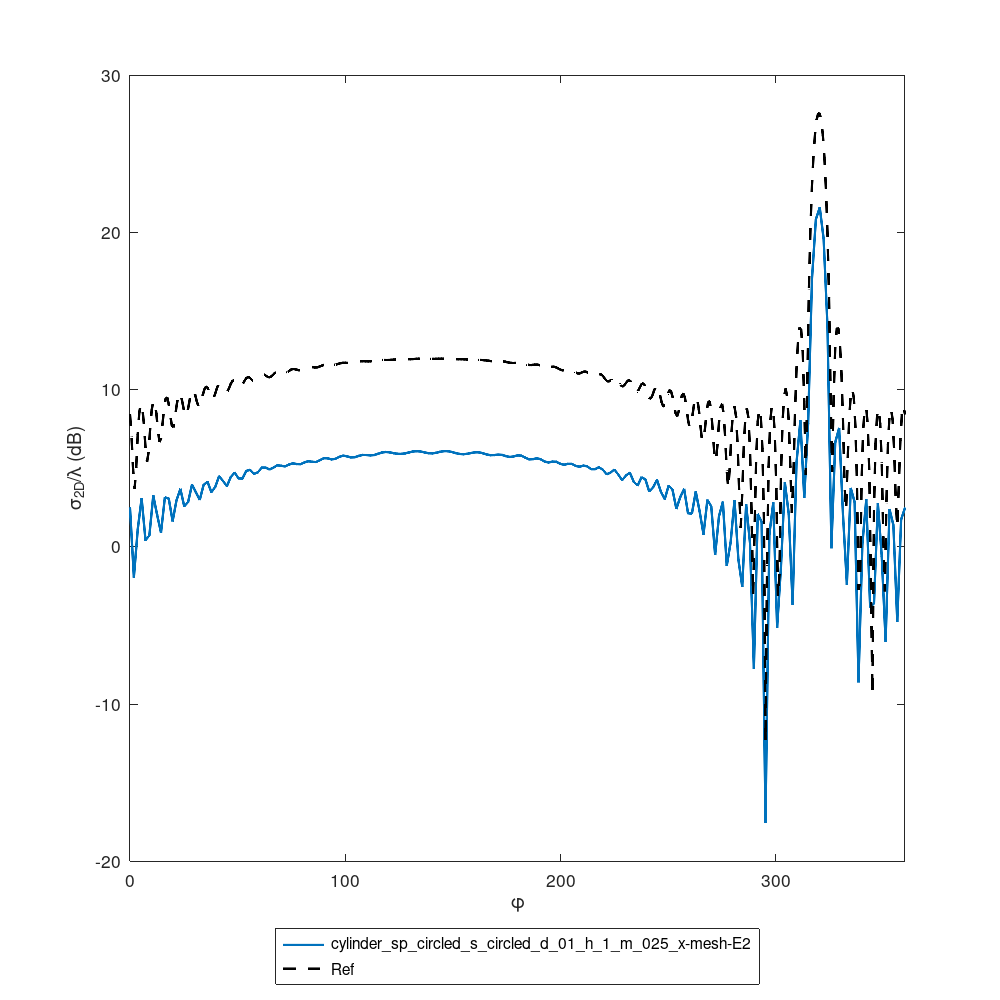
\includegraphics[width=\linewidth]{results/FF/cylD_01_H_1_M_025_X/epr1_TE.png}

\column{0.23\textwidth}

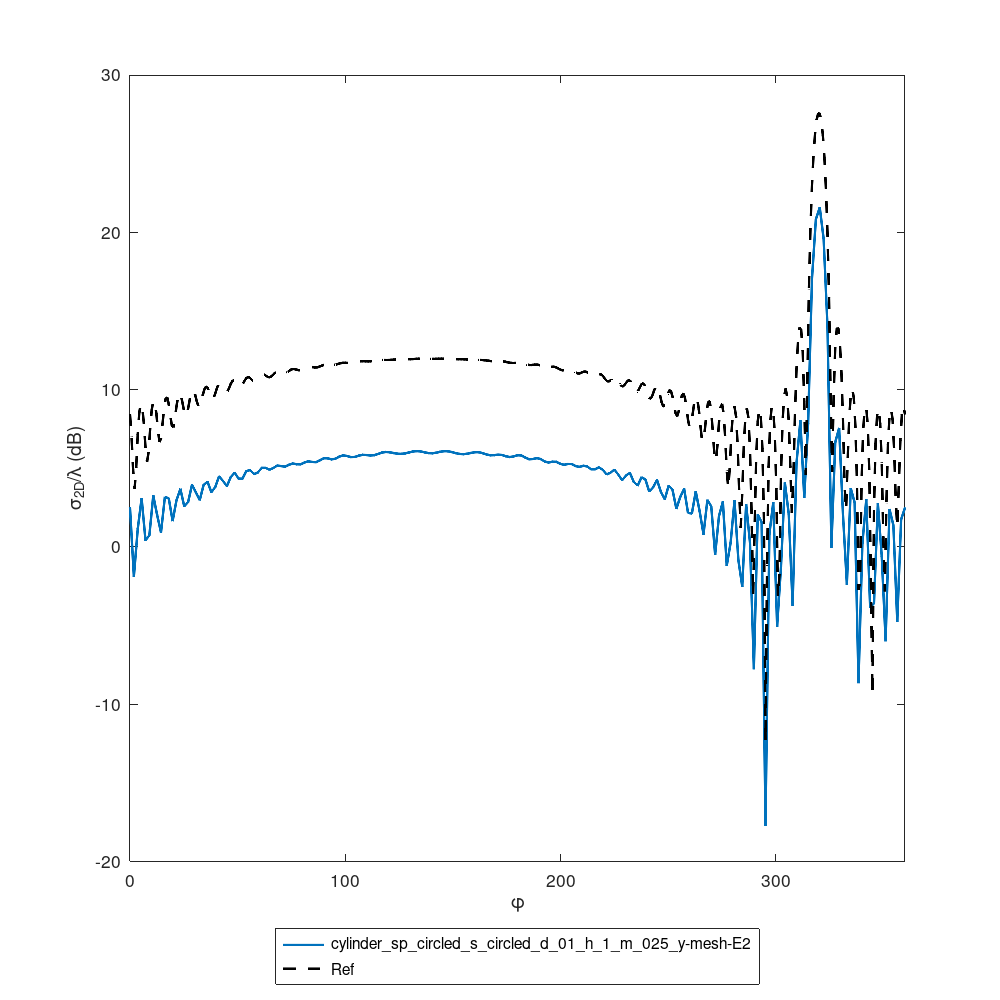
\includegraphics[width=\linewidth]{results/FF/cylD_01_H_1_M_025_Y/epr1_TE.png}

\column{0.23\textwidth}

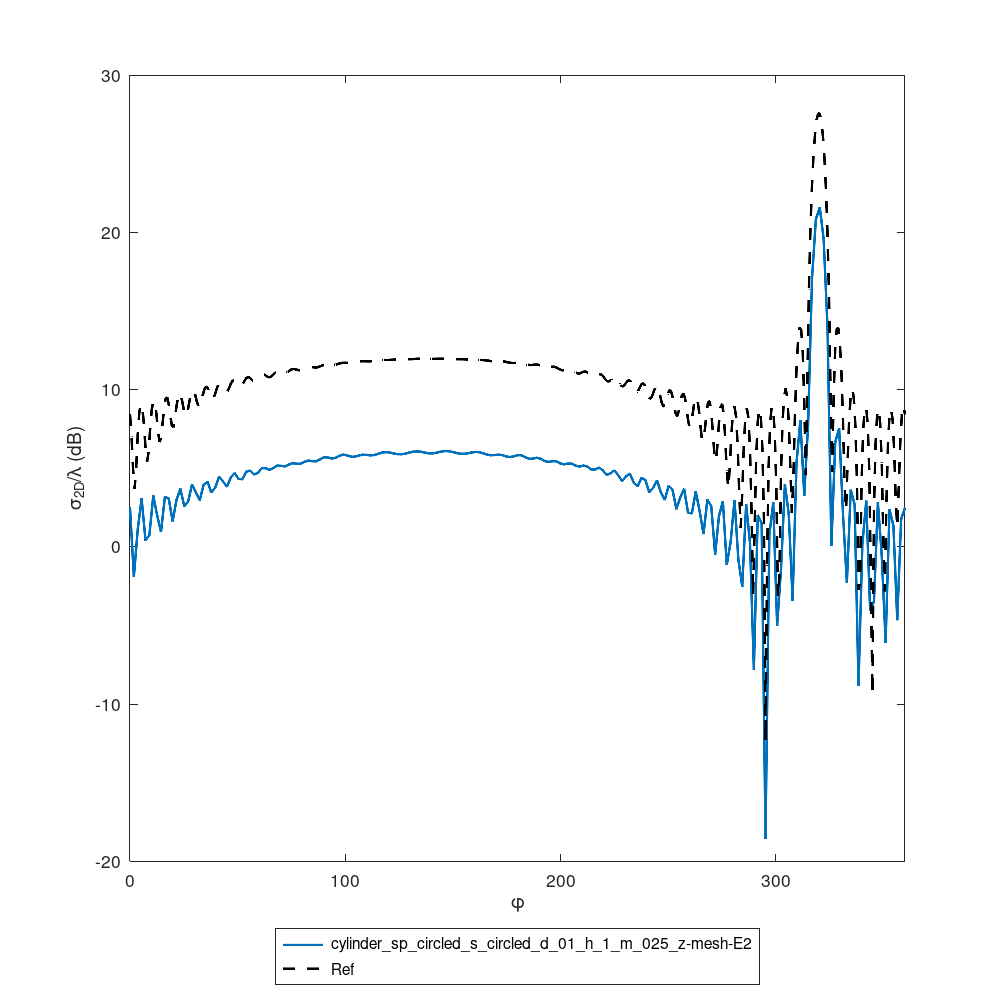
\includegraphics[width=\linewidth]{results/FF/cylD_01_H_1_M_025_Z/epr1_TE.png}

\column{0.23\textwidth}

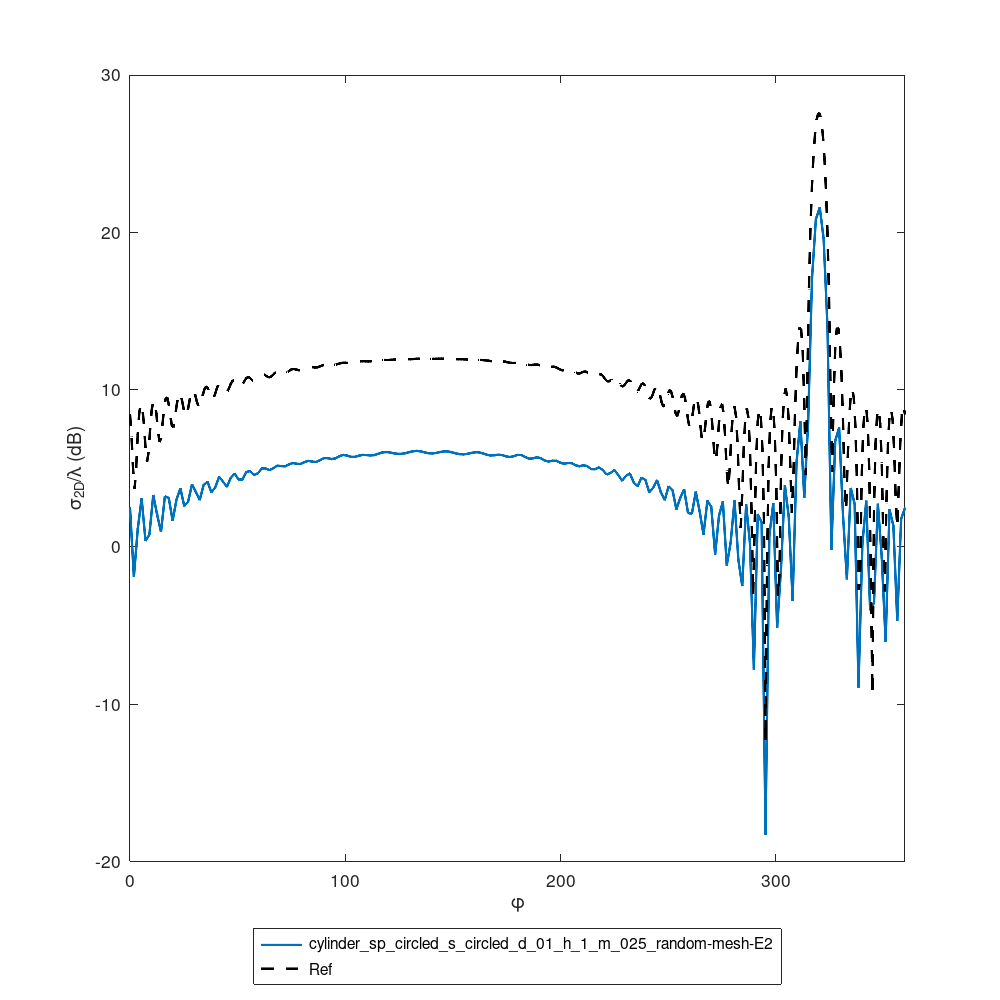
\includegraphics[width=\linewidth]{results/FF/cylD_01_H_1_M_025_RANDOM/epr1_TE.png}

\end{columns}

\vbs

Analytical curves and FEM curves agree except for a constant factor. 

Normalized bistatic-RCS:

\vbss

\begin{columns}
\column{0.23\textwidth}

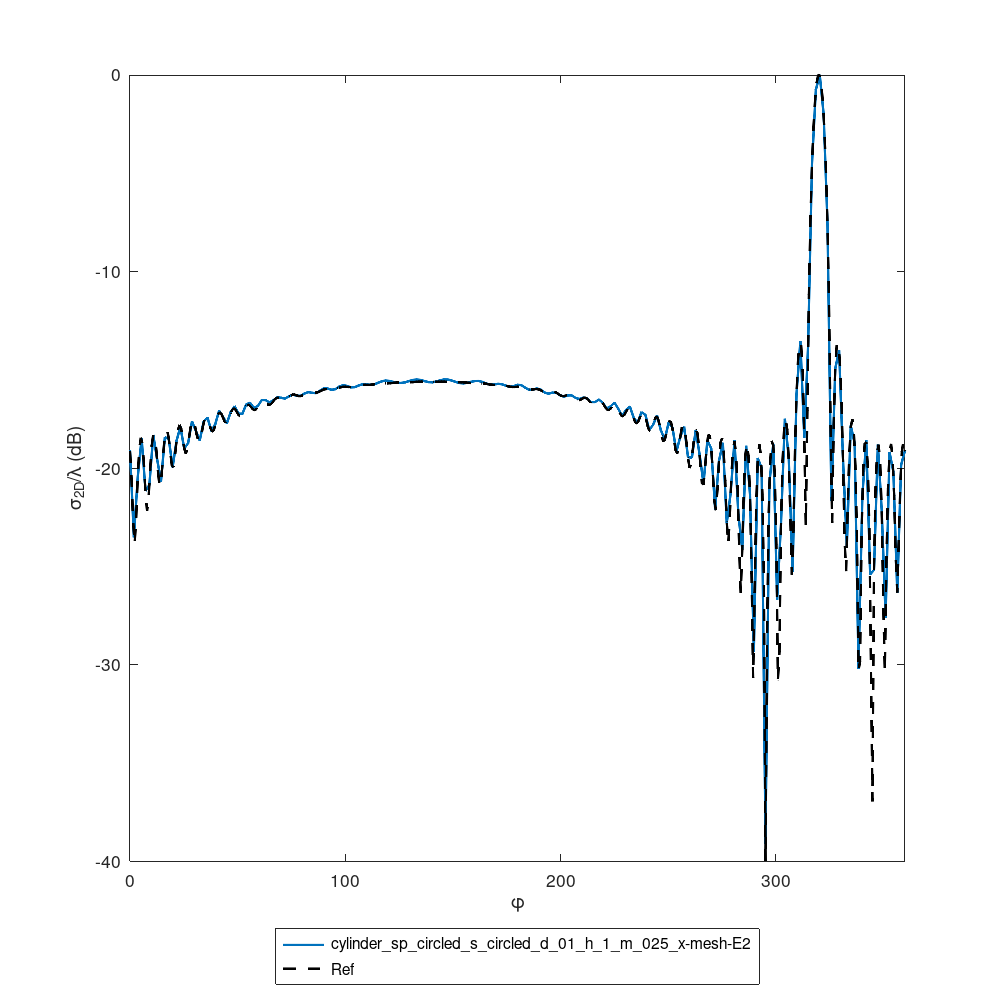
\includegraphics[width=\linewidth]{results/FF/cylD_01_H_1_M_025_X/epr1_TE_norm.png}

\column{0.23\textwidth}

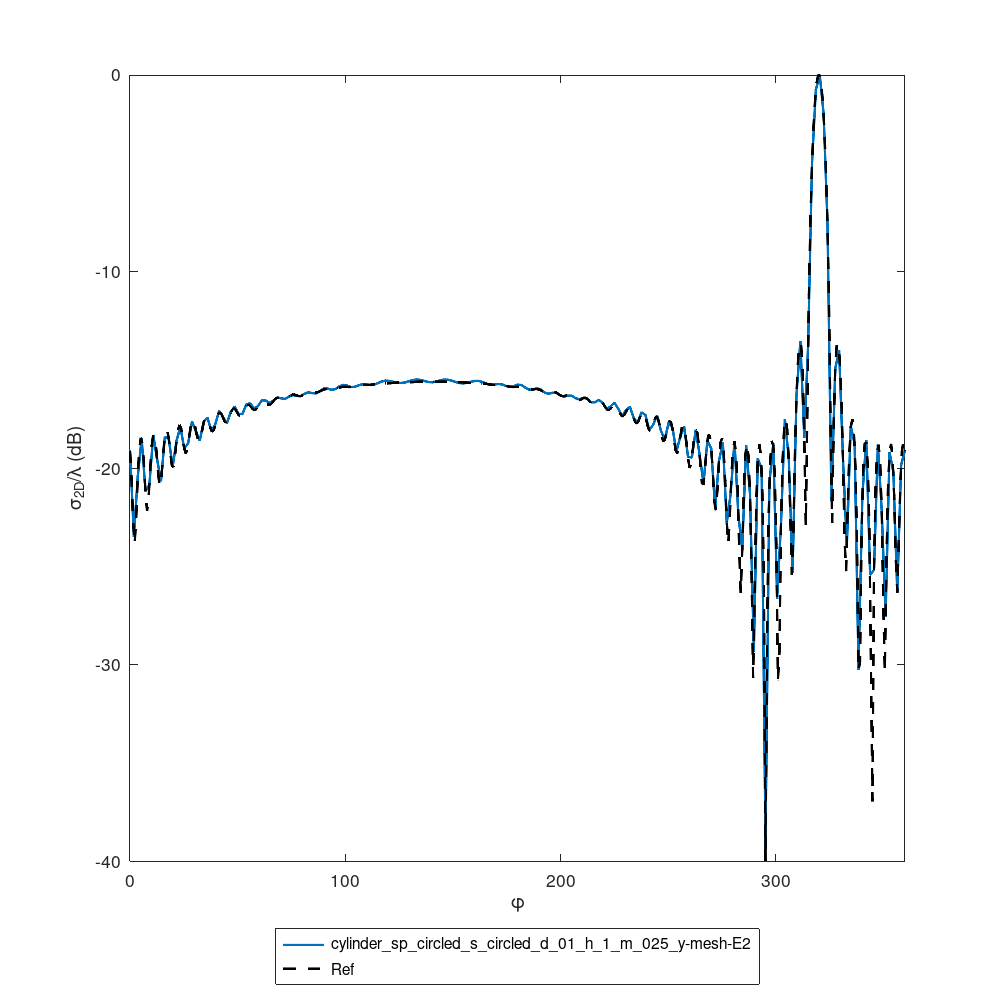
\includegraphics[width=\linewidth]{results/FF/cylD_01_H_1_M_025_Y/epr1_TE_norm.png}

\column{0.23\textwidth}

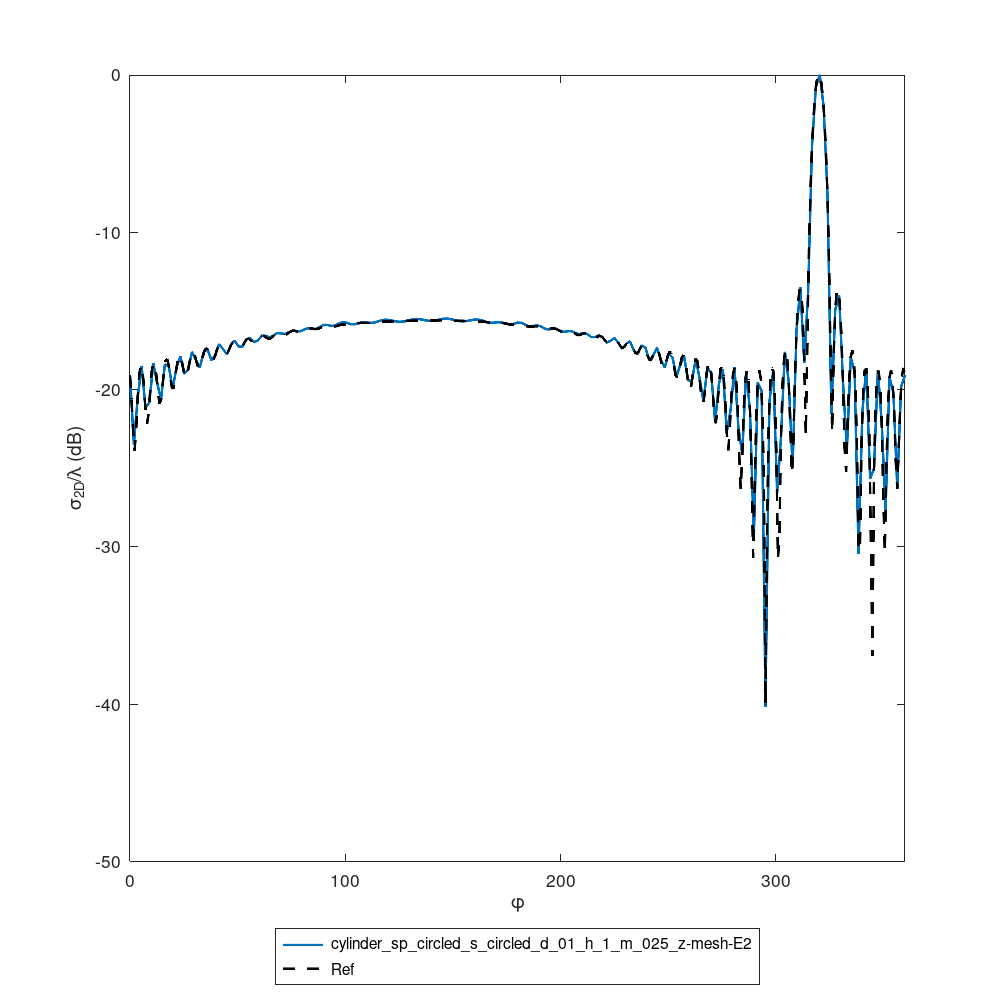
\includegraphics[width=\linewidth]{results/FF/cylD_01_H_1_M_025_Z/epr1_TE_norm.png}

\column{0.23\textwidth}

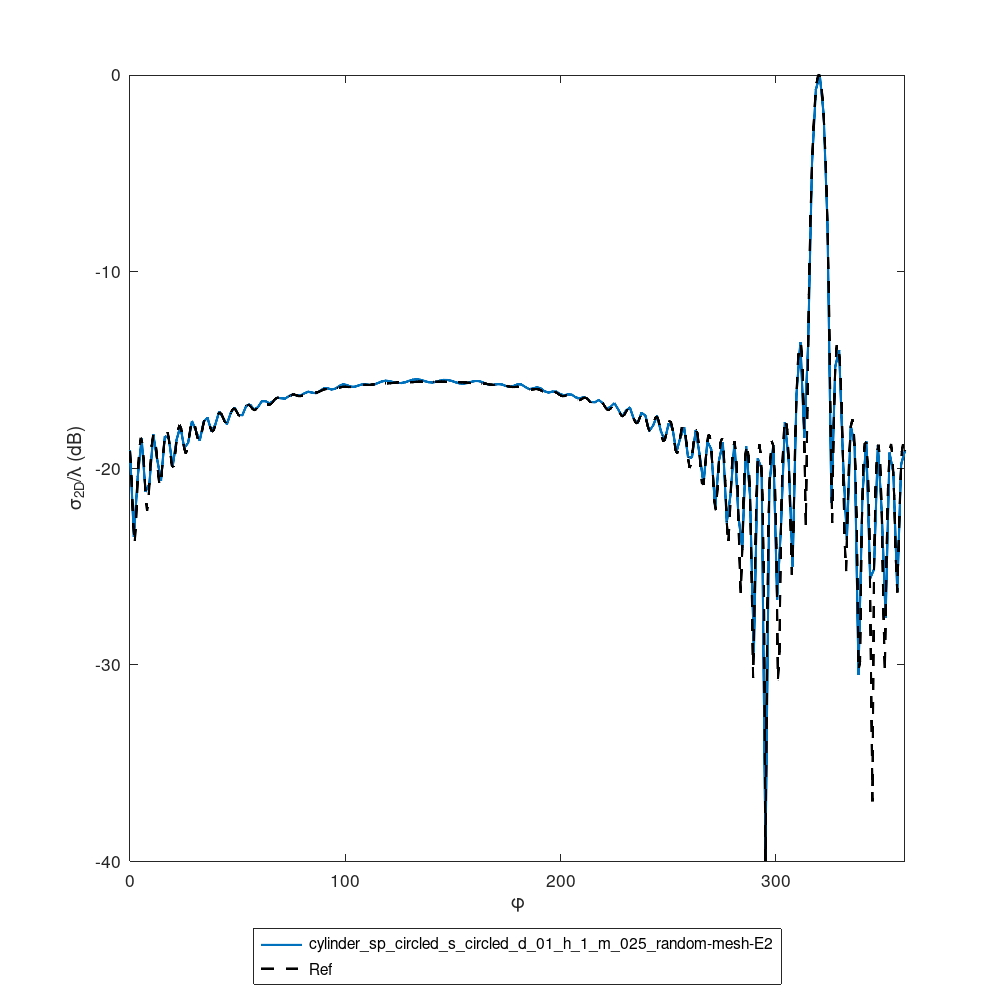
\includegraphics[width=\linewidth]{results/FF/cylD_01_H_1_M_025_RANDOM/epr1_TE_norm.png}

\end{columns}



\end{frame}

%%%%%%%%%%%%%%%%%%%%%%%%%%%%%%%%%%%%%%%%

\begin{frame}{TM polarization, $\varepsilon_r=8$}

\begin{columns}
\column{0.23\textwidth}

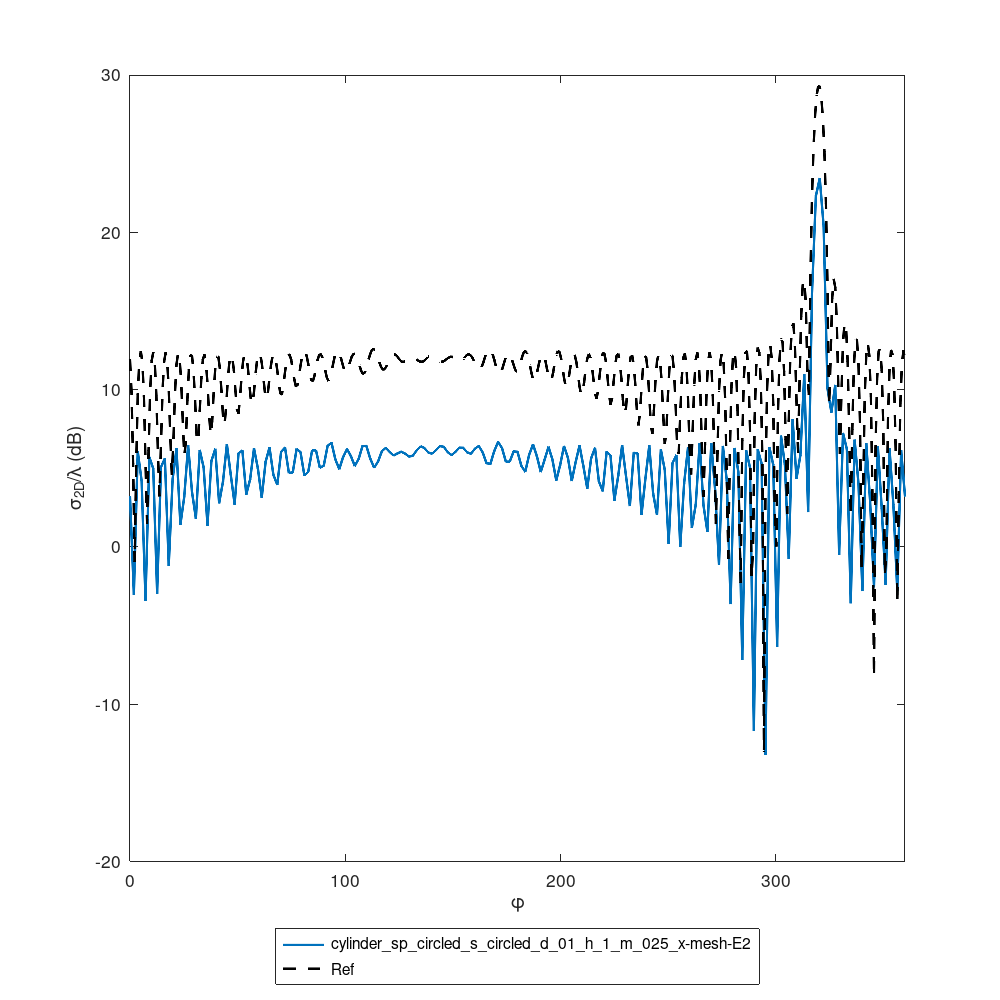
\includegraphics[width=\linewidth]{results/FF/cylD_01_H_1_M_025_X/epr8_TM.png}

\column{0.23\textwidth}

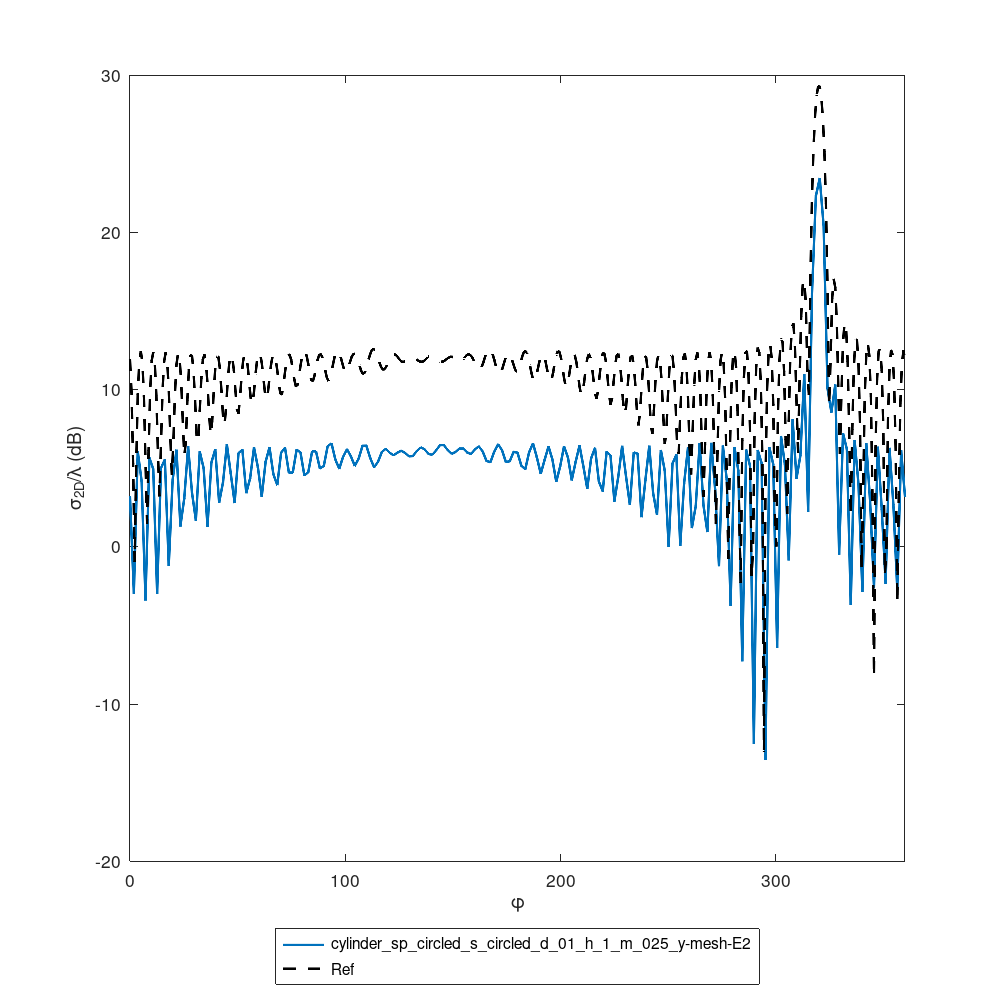
\includegraphics[width=\linewidth]{results/FF/cylD_01_H_1_M_025_Y/epr8_TM.png}

\column{0.23\textwidth}

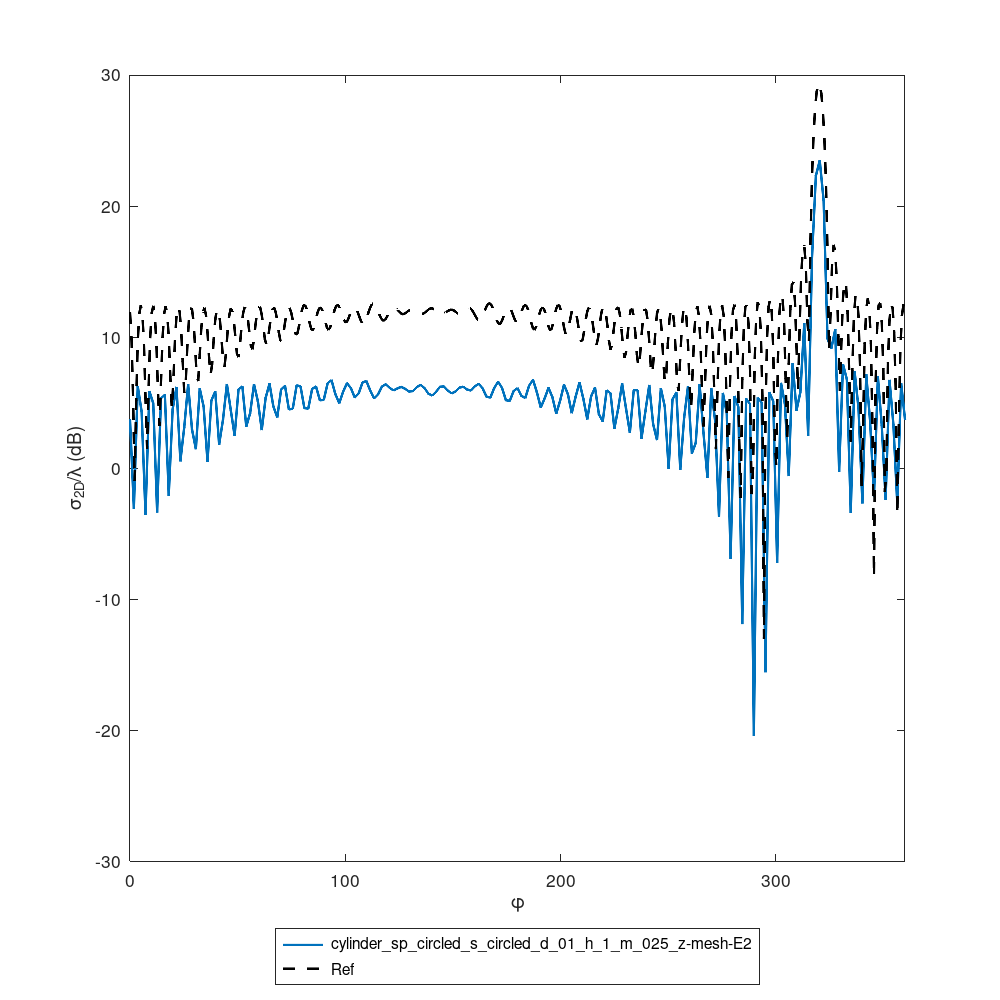
\includegraphics[width=\linewidth]{results/FF/cylD_01_H_1_M_025_Z/epr8_TM.png}

\column{0.23\textwidth}

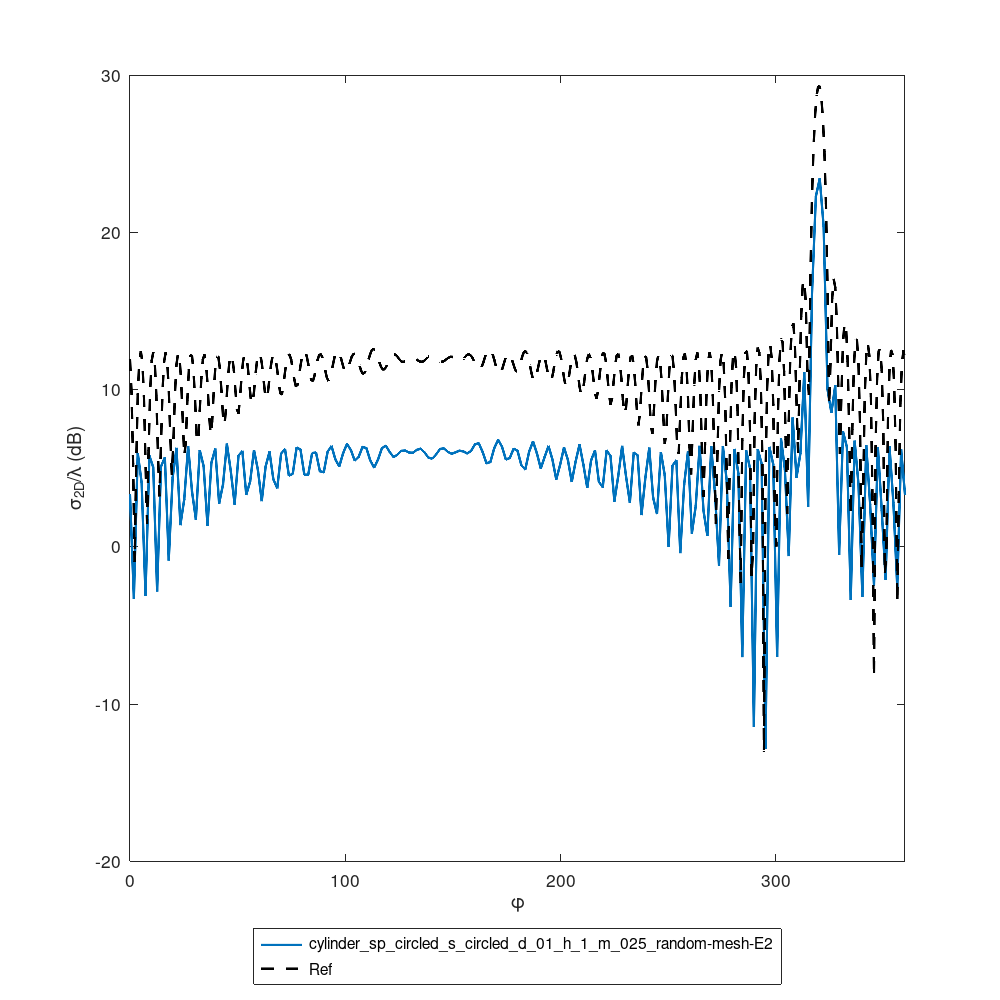
\includegraphics[width=\linewidth]{results/FF/cylD_01_H_1_M_025_RANDOM/epr8_TM.png}

\end{columns}

\vbs

Analytical curves and FEM curves agree (minor discrepancies) except for a constant factor. 

Normalized bistatic-RCS:

\vbss

\begin{columns}
\column{0.23\textwidth}

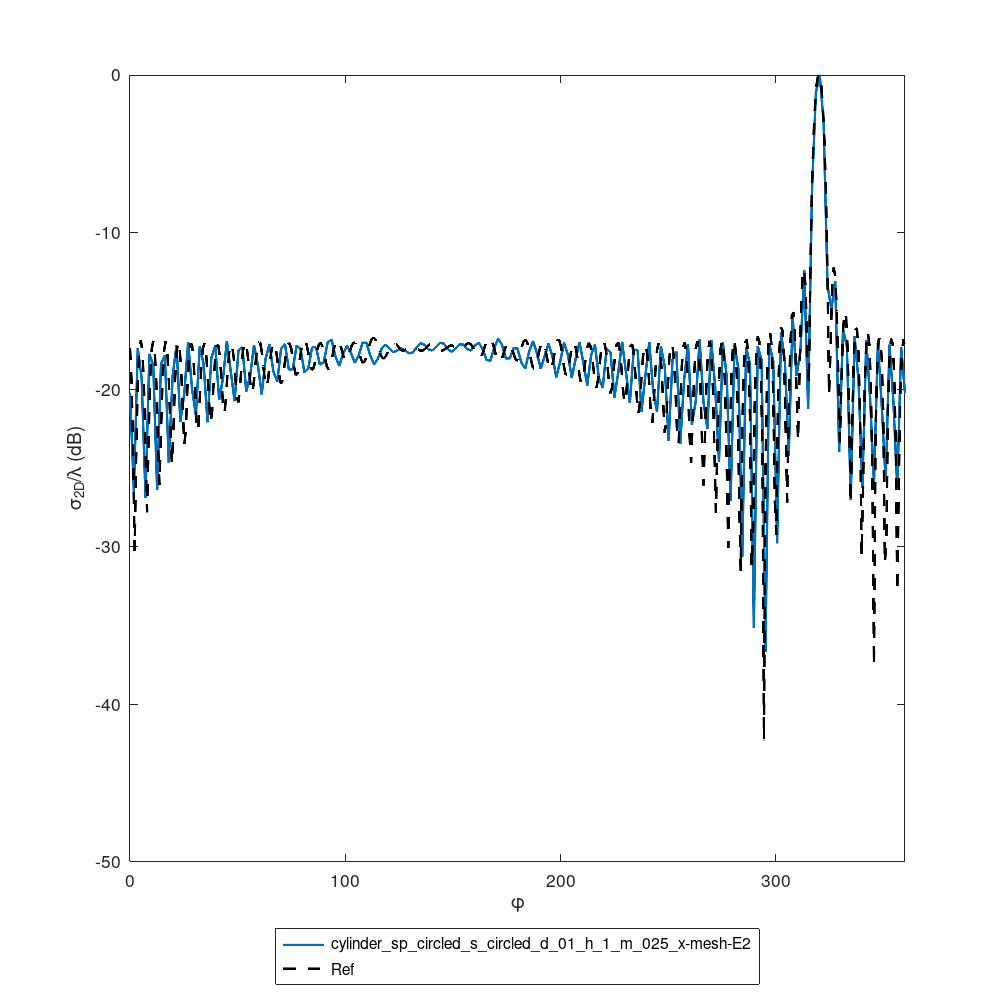
\includegraphics[width=\linewidth]{results/FF/cylD_01_H_1_M_025_X/epr8_TM_norm.png}

\column{0.23\textwidth}

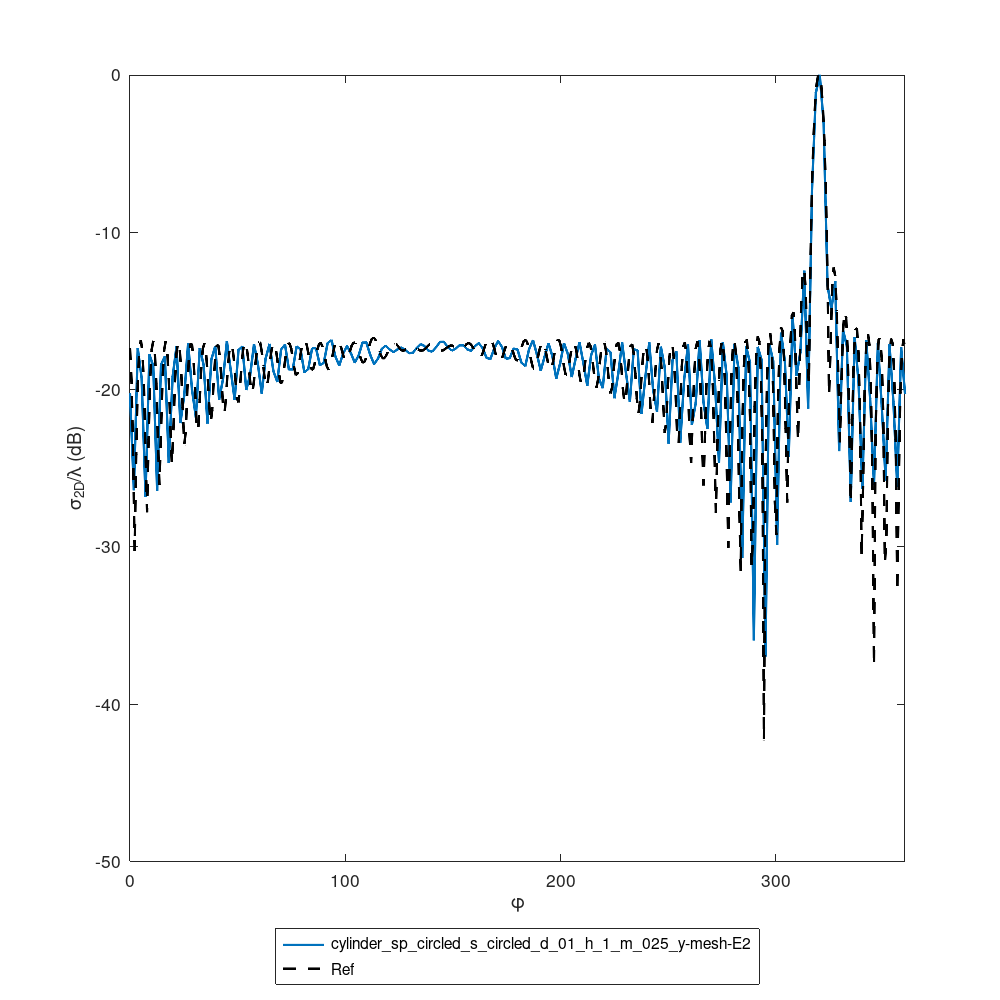
\includegraphics[width=\linewidth]{results/FF/cylD_01_H_1_M_025_Y/epr8_TM_norm.png}

\column{0.23\textwidth}

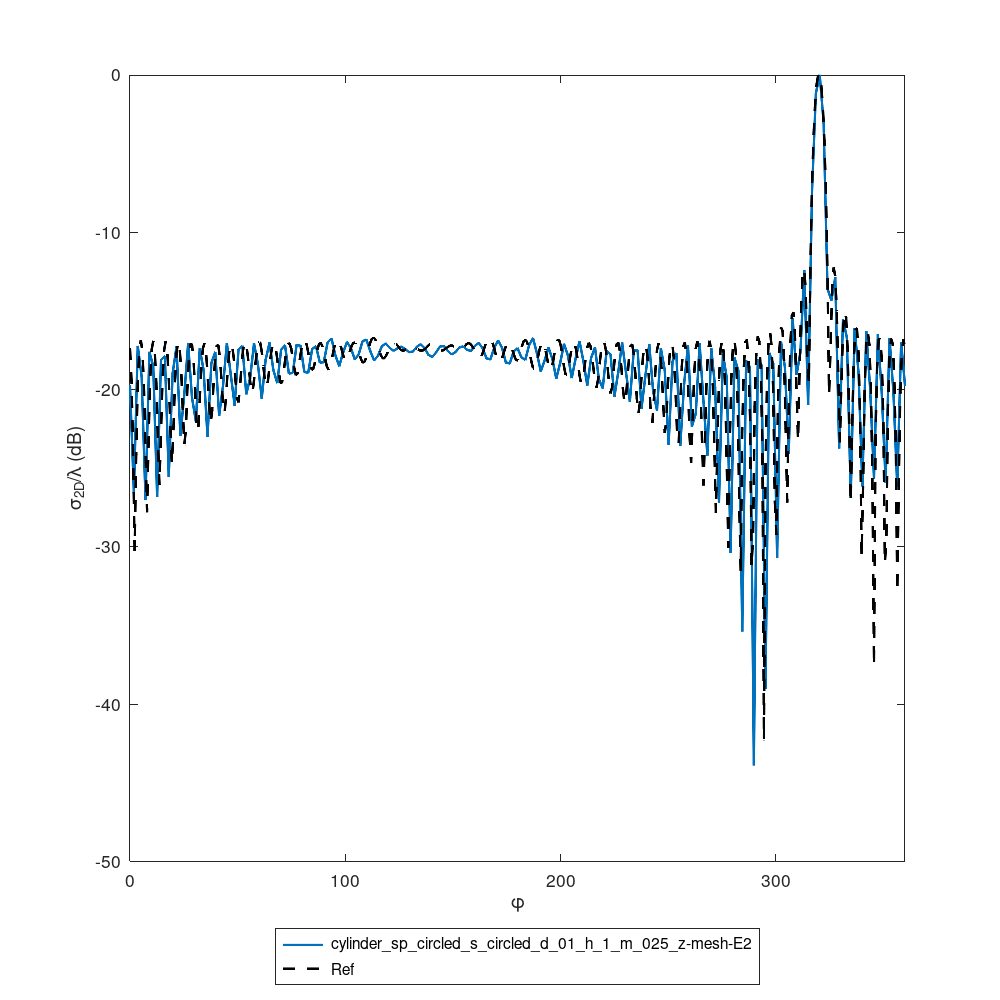
\includegraphics[width=\linewidth]{results/FF/cylD_01_H_1_M_025_Z/epr8_TM_norm.png}

\column{0.23\textwidth}

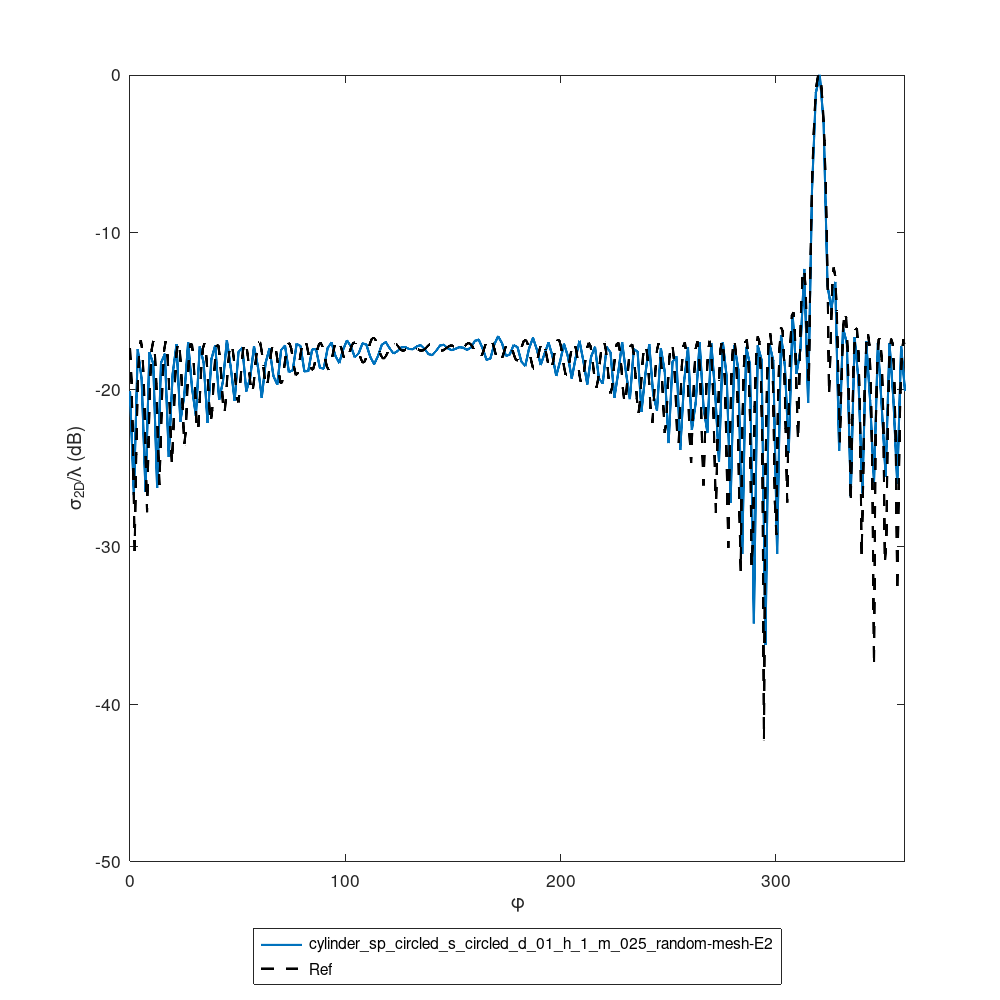
\includegraphics[width=\linewidth]{results/FF/cylD_01_H_1_M_025_RANDOM/epr8_TM_norm.png}

\end{columns}



\end{frame}


%%%%%%%%%%%%%%%%%%%%%%%%%%%%%%%%%%%%%%%%

\begin{frame}{TE polarization, $\varepsilon_r=2$}

\begin{columns}
\column{0.23\textwidth}

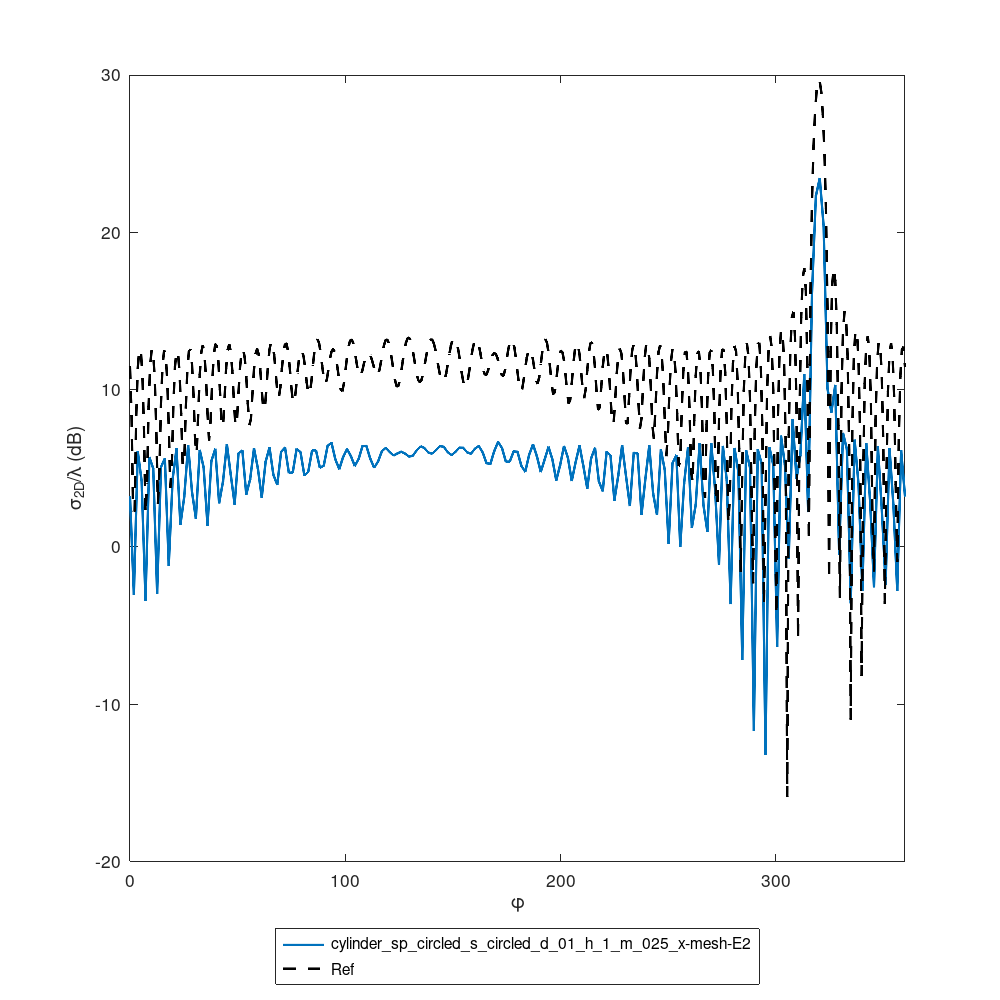
\includegraphics[width=\linewidth]{results/FF/cylD_01_H_1_M_025_X/epr2_TE.png}

\column{0.23\textwidth}

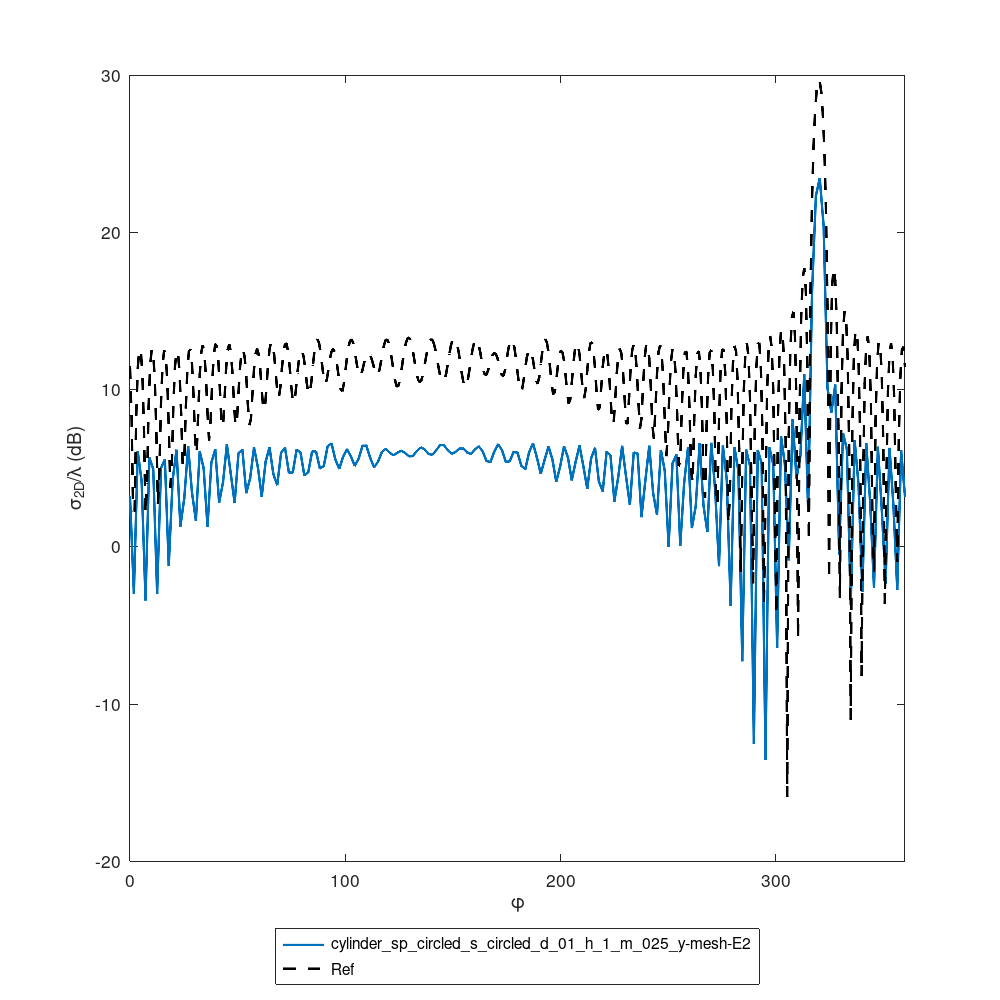
\includegraphics[width=\linewidth]{results/FF/cylD_01_H_1_M_025_Y/epr2_TE.png}

\column{0.23\textwidth}

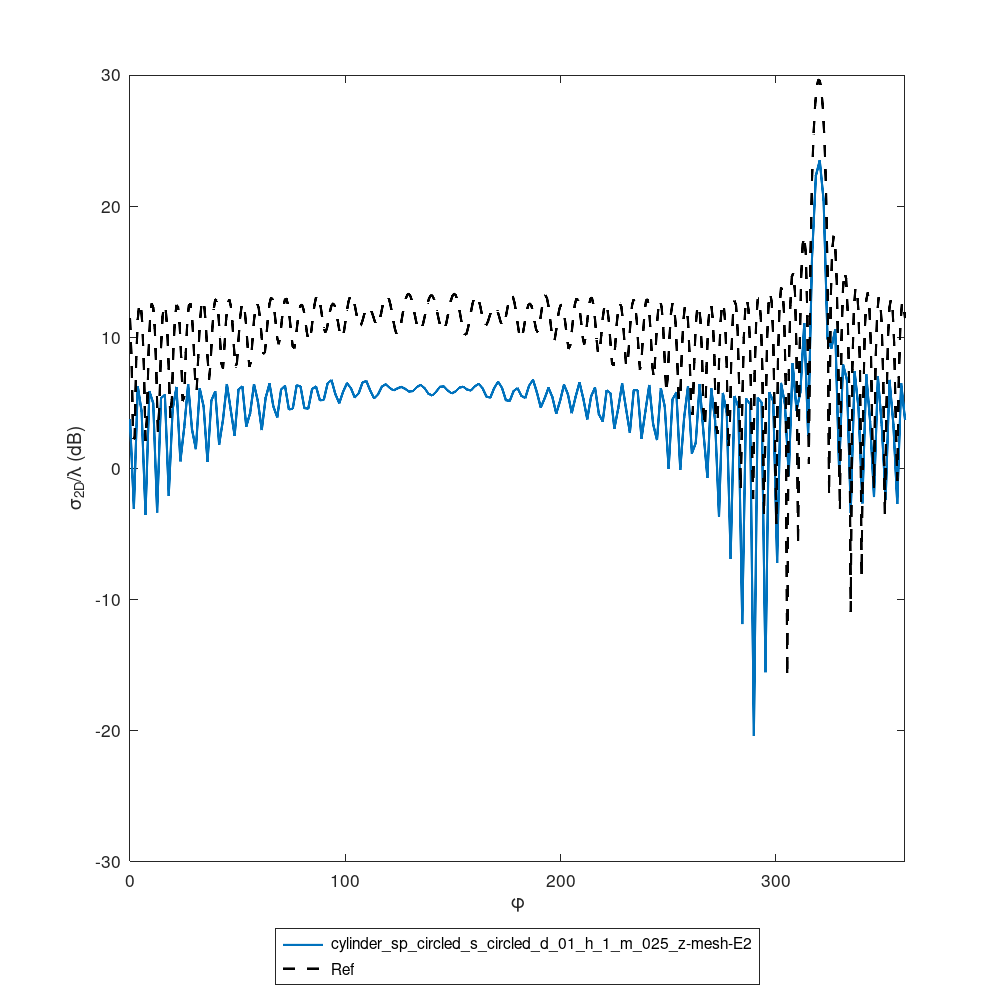
\includegraphics[width=\linewidth]{results/FF/cylD_01_H_1_M_025_Z/epr2_TE.png}

\column{0.23\textwidth}

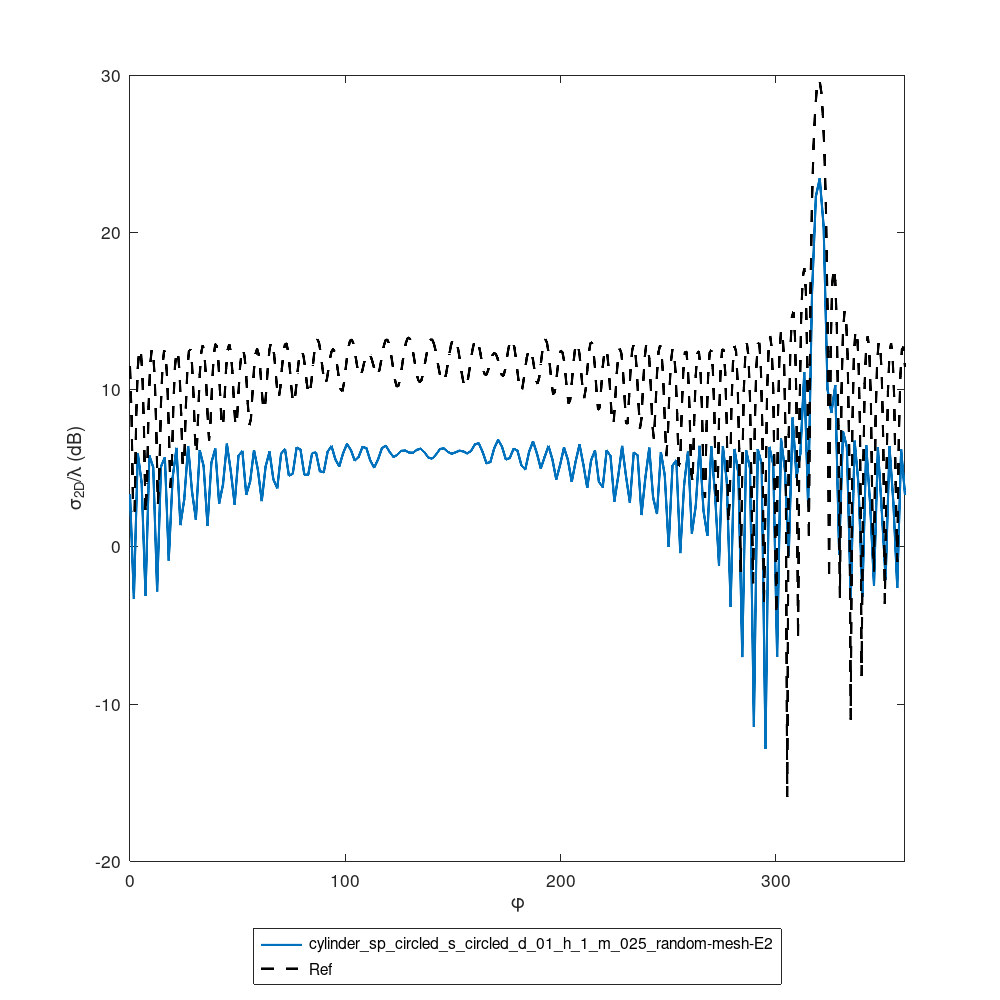
\includegraphics[width=\linewidth]{results/FF/cylD_01_H_1_M_025_RANDOM/epr2_TE.png}

\end{columns}

\vbs

Analytical curves and FEM curves agree (some discrepancies) except for a constant factor. 

Normalized bistatic-RCS:

\vbss

\begin{columns}
\column{0.23\textwidth}

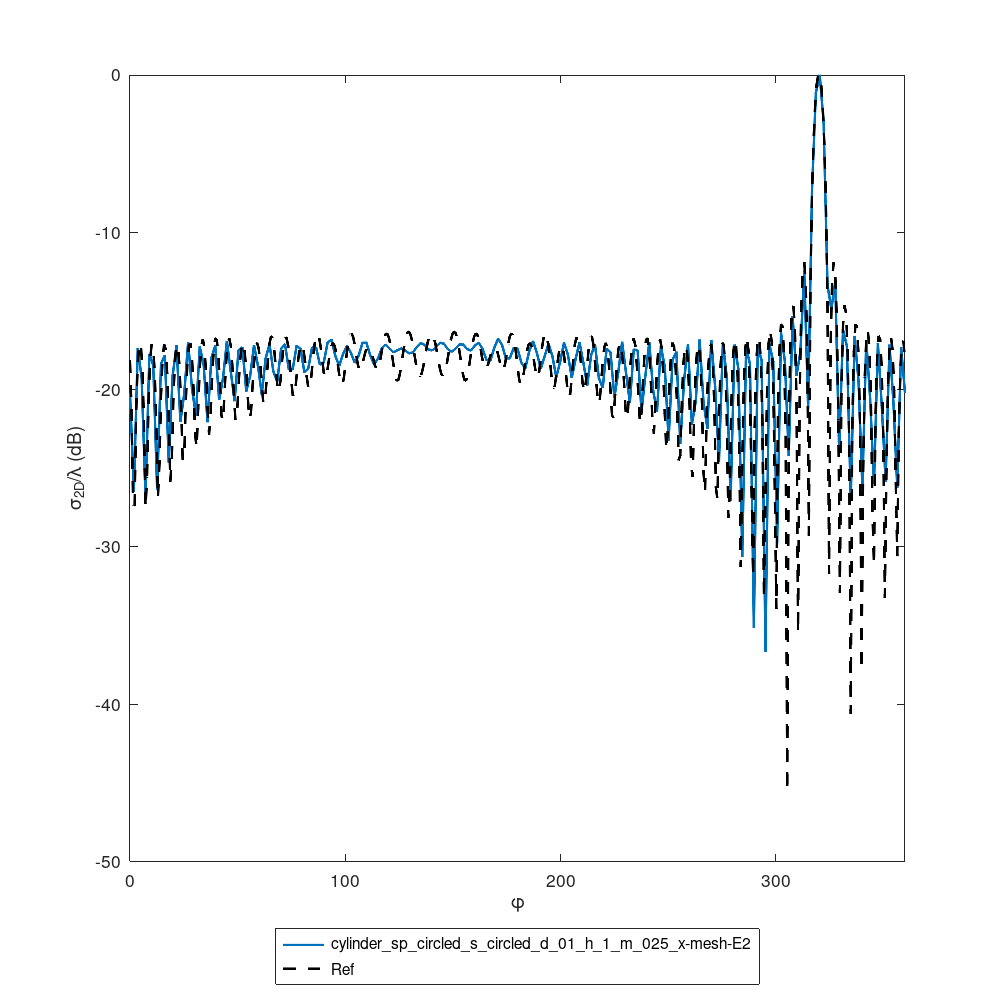
\includegraphics[width=\linewidth]{results/FF/cylD_01_H_1_M_025_X/epr2_TE_norm.png}

\column{0.23\textwidth}

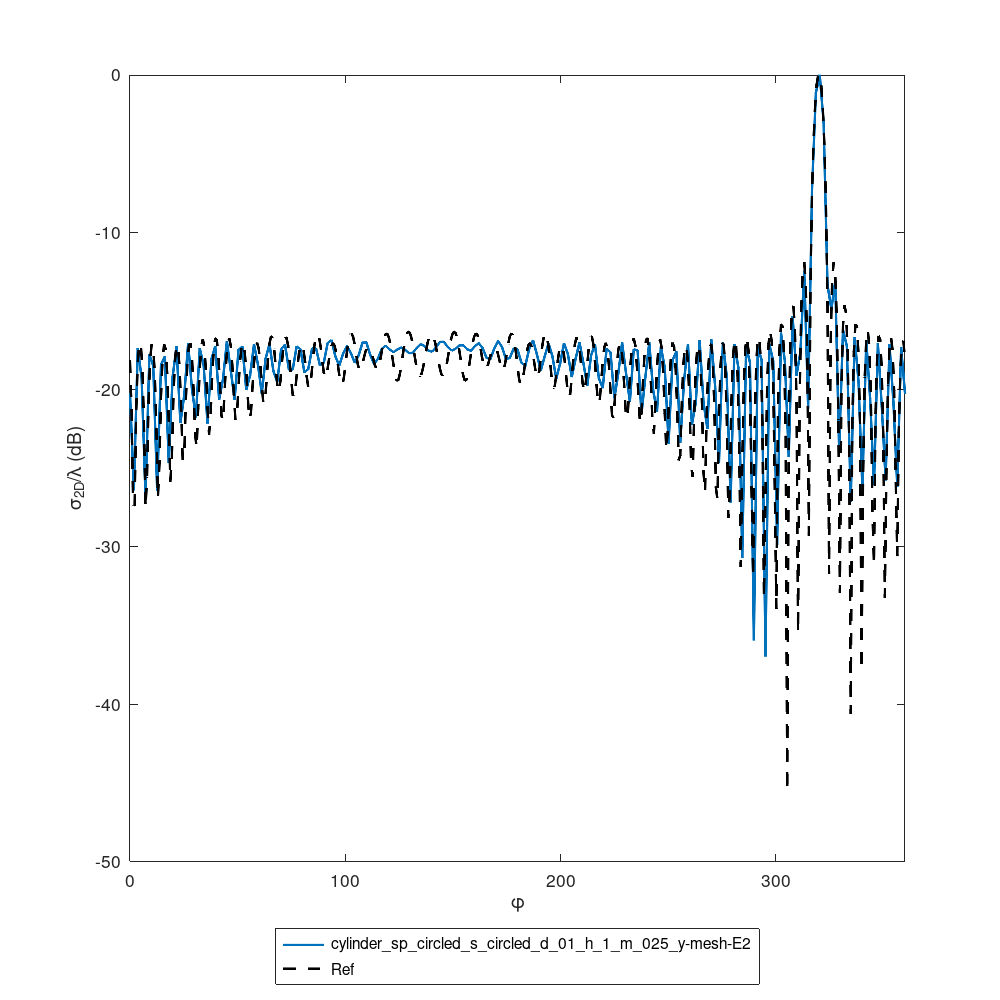
\includegraphics[width=\linewidth]{results/FF/cylD_01_H_1_M_025_Y/epr2_TE_norm.png}

\column{0.23\textwidth}

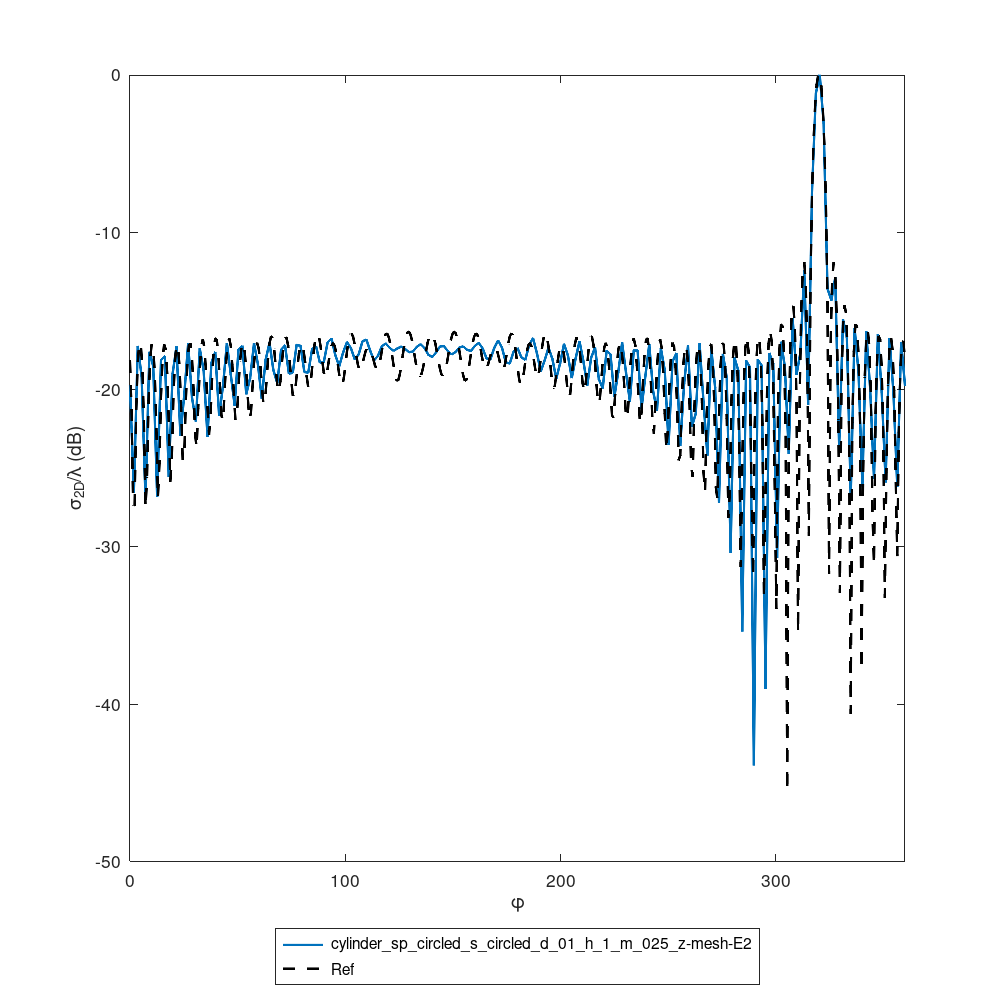
\includegraphics[width=\linewidth]{results/FF/cylD_01_H_1_M_025_Z/epr2_TE_norm.png}

\column{0.23\textwidth}

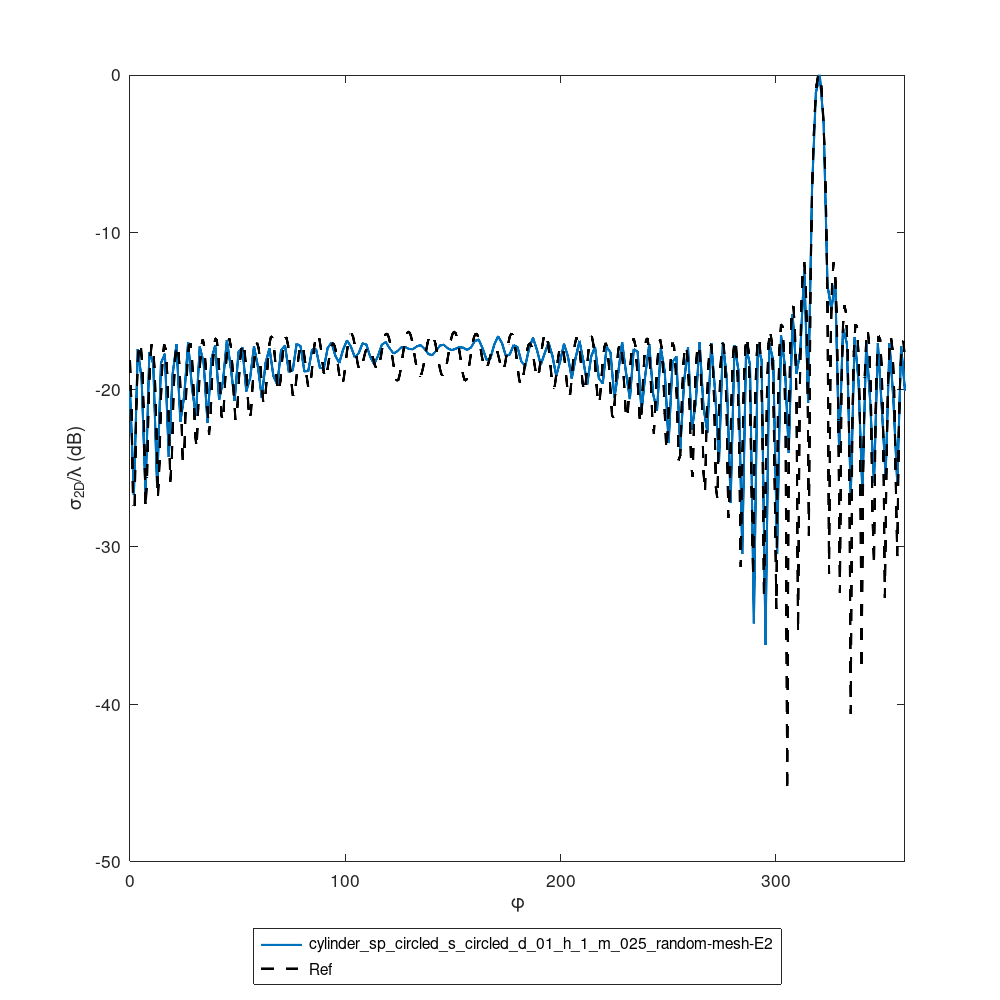
\includegraphics[width=\linewidth]{results/FF/cylD_01_H_1_M_025_RANDOM/epr2_TE_norm.png}

\end{columns}

\end{frame}

%%%%%%%%%%%%%%%%%%%%%%%%%%%%%%%%%%%%%%%%

\begin{frame}{TE polarization, $\varepsilon_r=2$, $f=150$\, MHz}

\begin{columns}
\column{0.23\textwidth}

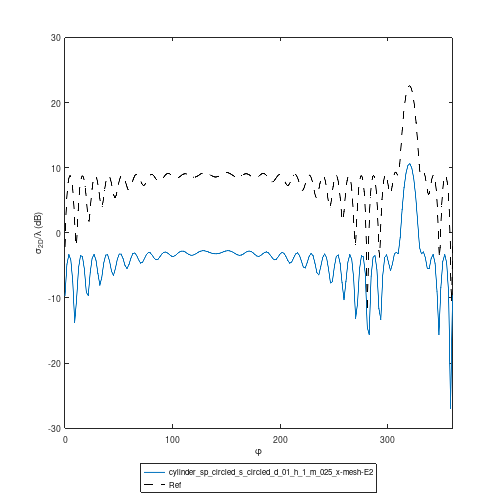
\includegraphics[width=\linewidth]{results/FF/cylD_01_H_1_M_025_X/epr2_TE_f150.png}

\column{0.23\textwidth}

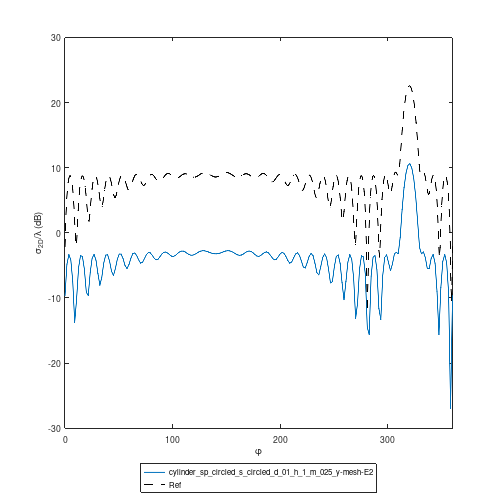
\includegraphics[width=\linewidth]{results/FF/cylD_01_H_1_M_025_Y/epr2_TE_f150.png}

\column{0.23\textwidth}

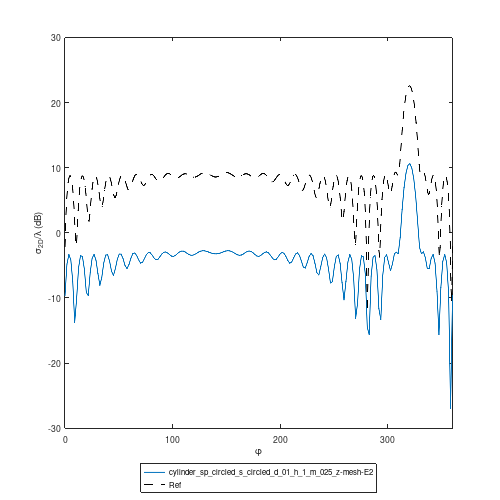
\includegraphics[width=\linewidth]{results/FF/cylD_01_H_1_M_025_Z/epr2_TE_f150.png}

\column{0.23\textwidth}

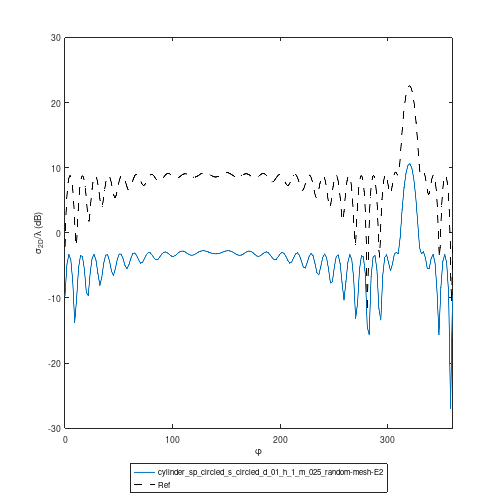
\includegraphics[width=\linewidth]{results/FF/cylD_01_H_1_M_025_RANDOM/epr2_TE_f150.png}

\end{columns}

\vbs

For a smaller problem (same mesh, double wavelength), almost full agree.

Normalized bistatic-RCS:

\vbss

\begin{columns}
\column{0.23\textwidth}

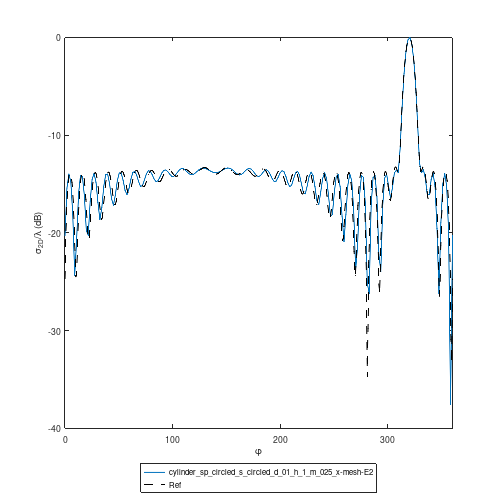
\includegraphics[width=\linewidth]{results/FF/cylD_01_H_1_M_025_X/epr2_TE_f150_norm.png}

\column{0.23\textwidth}

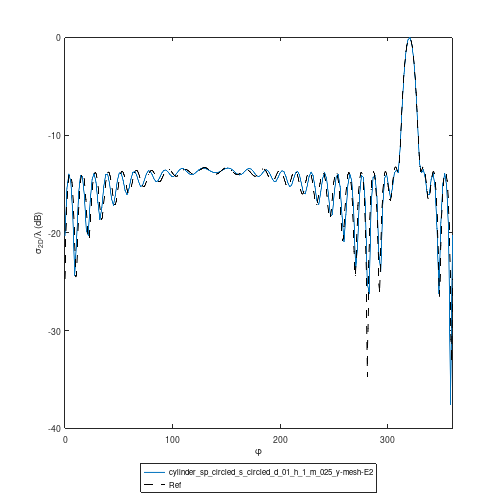
\includegraphics[width=\linewidth]{results/FF/cylD_01_H_1_M_025_Y/epr2_TE_f150_norm.png}

\column{0.23\textwidth}

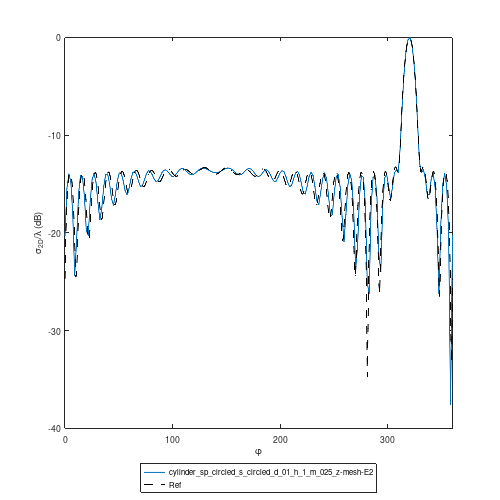
\includegraphics[width=\linewidth]{results/FF/cylD_01_H_1_M_025_Z/epr2_TE_f150_norm.png}

\column{0.23\textwidth}

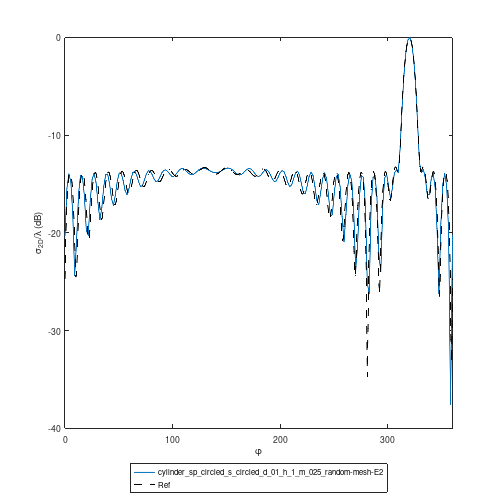
\includegraphics[width=\linewidth]{results/FF/cylD_01_H_1_M_025_RANDOM/epr2_TE_f150_norm.png}

\end{columns}

\end{frame}

%%%%%%%%%%%%%%%%%%%%%%%%%%%%%%%%%%%%%%%%

\begin{frame}{Effect of IIEE iterative method in Far Field}{TM polarization, $\varepsilon_r=1$, (reference case)}

Results for the following residual errors:
\begin{itemize}
\item \texttt{M1}: $10^{-1}$ (blue)
\item \texttt{M2}: $10^{-2}$ (red)
\item \texttt{M3}: $10^{-3}$ (orange)
\end{itemize}


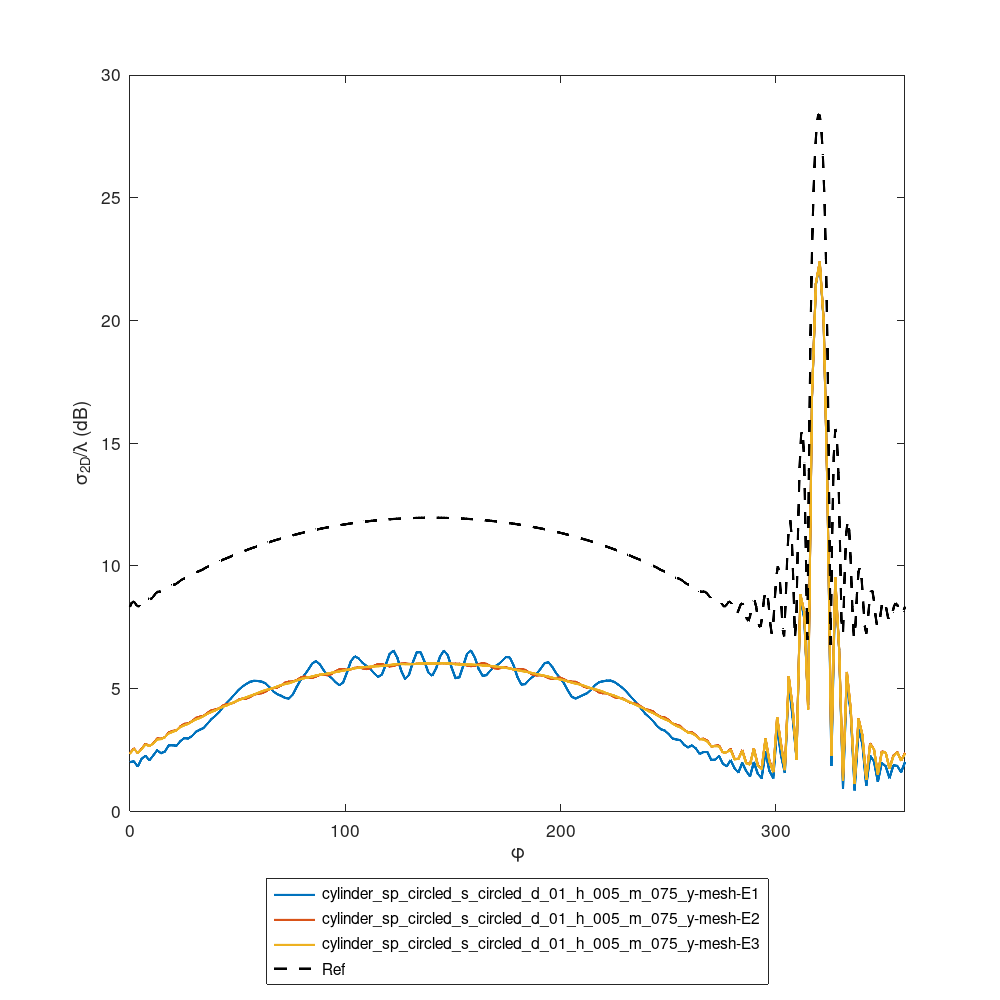
\includegraphics[width=0.45\linewidth]{results/FF/cylD_01_H_005_M_075_Y/iiee075.png}
\hfill
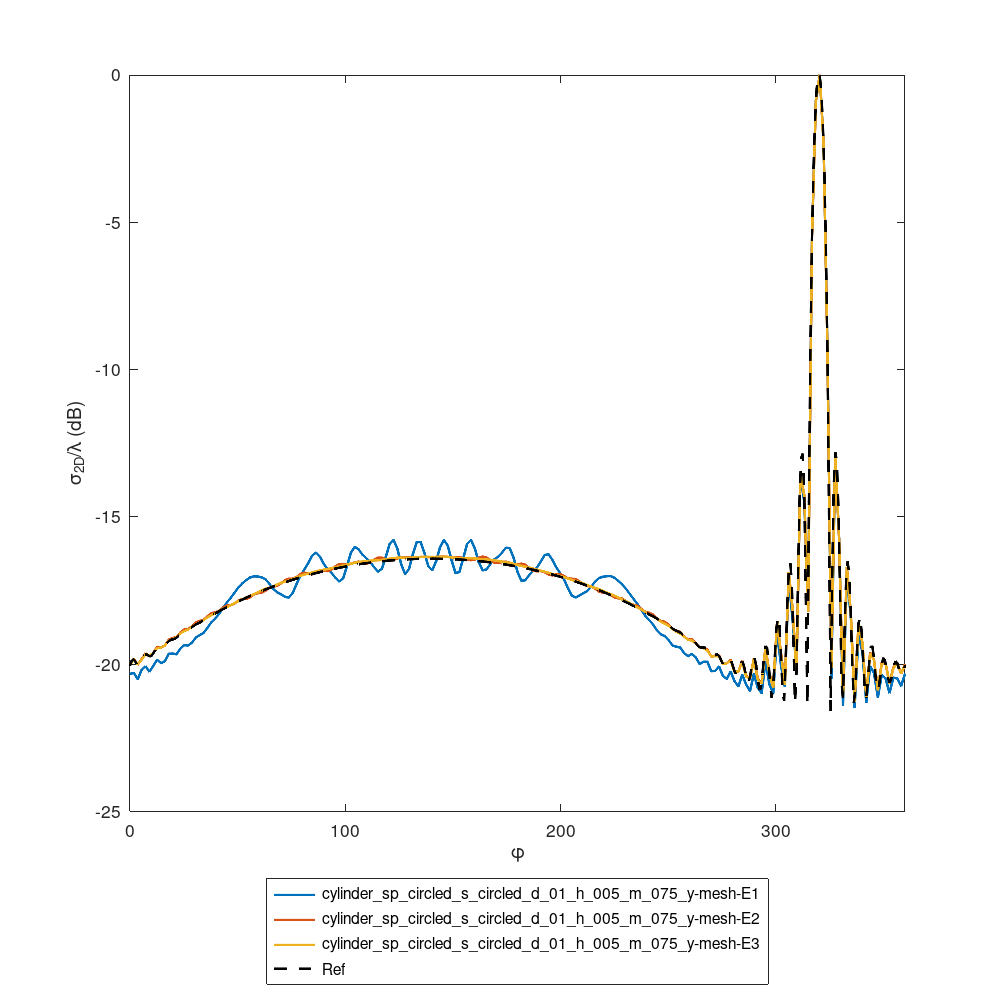
\includegraphics[width=0.45\linewidth]{results/FF/cylD_01_H_005_M_075_Y/iiee075_norm.png}


Note: Orange and red lines overlap. 

\end{frame}

  
% %%%%%%%%%%%%%%%%%%%%%%%%%%%%%%%%%%%%%%%%%%%%%%%%%%%%%%%%%%%%%%%
